\chapter{Higher inductive types}
\label{cha:hits}

\index{type!higher inductive|(}%
\indexsee{inductive!type!higher}{type, higher inductive}%
\indexsee{higher inductive type}{type, higher inductive}%

\section{Introduction}
\label{sec:intro-hits}

\index{generation!of a type, inductive|(}

Like the general inductive types we discussed in \autoref{cha:induction}, \emph{higher inductive types} are a general schema for defining new types generated by some constructors.
But unlike ordinary inductive types, in defining a higher inductive type we may have ``constructors'' which generate not only \emph{points} of that type, but also \emph{paths} and higher paths in that type.
\index{type!circle}%
\indexsee{circle type}{type,circle}%
For instance, we can consider the higher inductive type $\Sn^1$ generated by
\begin{itemize}
\item A point $\base:\Sn^1$, and
\item A path $\lloop : {\id[\Sn^1]\base\base}$.
\end{itemize}
This should be regarded as entirely analogous to the definition of, for instance, $\bool$, as being generated by
\begin{itemize}
\item A point $\bfalse:\bool$ and
\item A point $\btrue:\bool$,
\end{itemize}
or the definition of $\nat$ as generated by
\begin{itemize}
\item A point $0:\nat$ and
\item A function $\suc:\nat\to\nat$.
\end{itemize}
When we think of types as higher groupoids, the more general notion of ``generation'' is very natural:
since a higher groupoid is a ``multi-sorted object'' with paths and higher paths as well as points, we should allow ``generators'' in all dimensions.

We will refer to the ordinary sort of constructors (such as $\base$) as \define{point constructors}
\indexdef{constructor!point}%
\indexdef{point!constructor}%
or \emph{ordinary constructors}, and to the others (such as $\lloop$) as \define{path constructors}
\indexdef{constructor!path}%
\indexdef{path!constructor}%
or \emph{higher constructors}.
Each path constructor must specify the starting and ending point of the path, which we call its \define{source}
\indexdef{source!of a path constructor}%
and \define{target};
\indexdef{target!of a path constructor}%
for $\lloop$, both source and target are $\base$.

Note that a path constructor such as $\lloop$ generates a \emph{new} inhabitant of an identity type, which is not (at least, not \emph{a priori}) equal to any previously existing such inhabitant.
In particular, $\lloop$ is not \emph{a priori} equal to $\refl{\base}$ (although proving that they are definitely unequal takes a little thought; see \autoref{thm:loop-nontrivial}).
This is what distinguishes $\Sn^1$ from the ordinary inductive type \unit.

There are some important points to be made regarding this generalization.

\index{free!generation of an inductive type}%
First of all, the word ``generation'' should be taken seriously, in the same sense that a group can be freely generated by some set.
In particular, because a higher groupoid comes with \emph{operations} on paths and higher paths, when such an object is ``generated'' by certain constructors, the operations create more paths that do not come directly from the constructors themselves.
For instance, in the higher inductive type $\Sn^1$, the constructor $\lloop$ is not the only nontrivial path from $\base$ to $\base$; we have also ``$\lloop\ct\lloop$'' and ``$\lloop\ct\lloop\ct\lloop$'' and so on, as well as $\opp{\lloop}$, etc., all of which are different.
This may seem so obvious as to be not worth mentioning, but it is a departure from the behavior of ``ordinary'' inductive types, where one can expect to see nothing in the inductive type except what was ``put in'' directly by the constructors.

Secondly, this generation is really \emph{free} generation: higher inductive types do not technically allow us to impose ``axioms'', such as forcing ``$\lloop\ct\lloop$'' to equal $\refl{\base}$.
However, in the world of $\infty$-groupoids,%
\index{.infinity-groupoid@$\infty$-groupoid}
there is little difference between ``free generation'' and ``presentation'',
\index{presentation!of an infinity-groupoid@of an $\infty$-groupoid}%
\index{generation!of an infinity-groupoid@of an $\infty$-groupoid}%
since we can make two paths equal \emph{up to homotopy} by adding a new 2-di\-men\-sion\-al generator relating them (e.g.\ a path $\lloop\ct\lloop = \refl{\base}$ in $\base=\base$).
We do then, of course, have to worry about whether this new generator should satisfy its own ``axioms'', and so on, but in principle any ``presentation'' can be transformed into a ``free'' one by making axioms into constructors.
As we will see, by adding ``truncation constructors'' we can use higher inductive types to express classical notions such as group presentations as well.

Thirdly, even though a higher inductive type contains ``constructors'' which generate \emph{paths in} that type, it is still an inductive definition of a \emph{single} type.
In particular, as we will see, it is the higher inductive type itself which is given a universal property (expressed, as usual, by an induction principle), and \emph{not} its identity types.
The identity type of a higher inductive type retains the usual induction principle of any identity type (i.e.\ path induction), and does not acquire any new induction principle.

Thus, it may be nontrivial to identify the identity types of a higher inductive type in a concrete way, in contrast to how in \autoref{cha:basics} we were able to give explicit descriptions of the behavior of identity types under all the traditional type forming operations.
For instance, are there any paths from $\base$ to $\base$ in $\Sn^1$ which are not simply composites of copies of $\lloop$ and its inverse?
Intuitively, it seems that the answer should be no (and it is), but proving this is not trivial.
Indeed, such questions bring us rapidly to problems such as calculating the homotopy groups of spheres, a long-standing problem in algebraic topology for which no simple formula is known.
Homotopy type theory brings a new and powerful viewpoint to bear on such questions, but it also requires type theory to become as complex as the answers to these questions.

\index{dimension!of path constructors}%
Fourthly, the ``dimension'' of the constructors (i.e.\ whether they output points, paths, paths between paths, etc.)\ does not have a direct connection to which dimensions the resulting type has nontrivial homotopy in.
As a simple example, if an inductive type $B$ has a constructor of type $A\to B$, then any paths and higher paths in $A$ result in paths and higher paths in $B$, even though the constructor is not a ``higher'' constructor at all.
The same thing happens with higher constructors too: having a constructor of type $A\to (\id[B]xy)$ means not only that points of $A$ yield paths from $x$ to $y$ in $B$, but that paths in $A$ yield paths between these paths, and so on.
As we will see, this possibility is responsible for much of the power of higher inductive types.

On the other hand, it is even possible for constructors \emph{without} higher types in their inputs to generate ``unexpected'' higher paths.
For instance, in the 2-dimensional sphere $\Sn^2$ generated by
\symlabel{s2a}
\index{type!2-sphere}%
\begin{itemize}
\item A point $\base:\Sn^2$, and
\item A 2-dimensional path $\surf:\refl{\base} = \refl{\base}$ in ${\base=\base}$,
\end{itemize}
there is a nontrivial \emph{3-dimensional path} from $\refl{\refl{\base}}$ to itself.
Topologists will recognize this path as an incarnation of the \emph{Hopf fibration}.
From a category-theoretic point of view, this is the same sort of phenomenon as the fact mentioned above that $\Sn^1$ contains not only $\lloop$ but also $\lloop\ct\lloop$ and so on: it's just that in a \emph{higher} groupoid, there are \emph{operations} which raise dimension.
Indeed, we saw many of these operations back in \autoref{sec:equality}: the associativity and unit laws are not just properties, but operations, whose inputs are 1-paths and whose outputs are 2-paths.

\index{generation!of a type, inductive|)}%

% In US Trade format it wants a page break here but then it stretches the above itemize,
% so we give it some stretchable space to use if it wants to.
\vspace*{0pt plus 20ex}

\section{Induction principles and dependent paths}
\label{sec:dependent-paths}

When we describe a higher inductive type such as the circle as being generated by certain constructors, we have to explain what this means by giving rules analogous to those for the basic type constructors from \autoref{cha:typetheory}.
The constructors themselves give the \emph{introduction} rules, but it requires a bit more thought to explain the \emph{elimination} rules, i.e.\ the induction and recursion principles.
In this book we do not attempt to give a general formulation of what constitutes a ``higher inductive definition'' and how to extract the elimination rule from such a definition --- indeed, this is a subtle question and the subject of current research.
Instead we will rely on some general informal discussion and numerous examples.

\index{type!circle}%
\index{recursion principle!for S1@for $\Sn^1$}%
The recursion principle is usually easy to describe: given any type equipped with the same structure with which the constructors equip the higher inductive type in question, there is a function which maps the constructors to that structure.
For instance, in the case of $\Sn^1$, the recursion principle says that given any type $B$ equipped with a point $b:B$ and a path $\ell:b=b$, there is a function $f:\Sn^1\to B$ such that $f(\base)=b$ and $\apfunc f (\lloop) = \ell$.

\index{computation rule!for S1@for $\Sn^1$}%
\index{equality!definitional}%
The latter two equalities are the \emph{computation rules}.
\index{computation rule!for higher inductive types|(}%
\index{computation rule!propositional|(}%
There is, however, a question of whether these computation rules are judgmental\index{judgmental equality} equalities or propositional equalities (paths).
For ordinary inductive types, we had no qualms about making them judgmental, although we saw in \autoref{cha:induction} that making them propositional would still yield the same type up to equivalence.
In the ordinary case, one may argue that the computation rules are really \emph{definitional} equalities, in the intuitive sense described in the Introduction.

\index{equality!judgmental}%
For higher inductive types, this is less clear. %, and it is likewise less clear to what extent these equalities can be made judgmental in the known set-theoretic models.
Moreover, since the operation $\apfunc f$ is not really a fundamental part of the type theory, but something that we \emph{defined} using the induction principle of identity types (and which we might have defined in some other, equivalent, way), it seems inappropriate to refer to it explicitly in a \emph{judgmental} equality.
Judgmental equalities are part of the deductive system, which should not depend on particular choices of definitions that we may make \emph{within} that system.
There are also semantic and implementation issues to consider; see the Notes.

It does seem unproblematic to make the computational rules for the \emph{point} constructors of a higher inductive type judgmental.
In the example above, this means we have $f(\base)\jdeq b$, judgmentally.
This choice facilitates a computational view of higher inductive types.
Moreover, it also greatly simplifies our lives, since otherwise the second computation rule $\apfunc f (\lloop) = \ell$ would not even be well-typed as a propositional equality; we would have to compose one side or the other with the specified identification of $f(\base)$ with $b$.
(Such problems do arise eventually, of course, when we come to talk about paths of higher dimension, but that will not be of great concern to us here.
See also \autoref{sec:hubs-spokes}.)
Thus, we take the computation rules for point constructors to be judgmental, and those for paths and higher paths to be propositional.%
\footnote{In particular, in the language of \autoref{sec:types-vs-sets}, this means that our higher inductive types are a mix of \emph{rules} (specifying how we can introduce such types and their elements, their induction principle, and their computation rules for point constructors) and \emph{axioms} (the computation rules for path constructors, which assert that certain identity types are inhabited by otherwise unspecified terms).
We may hope that eventually, there will be a better type theory in which higher inductive types, like univalence, will be presented using only rules and no axioms.%
\indexfoot{axiom!versus rules}%
\indexfoot{rule!versus axioms}%
}

\begin{rmk}\label{rmk:defid}
Recall that for ordinary inductive types, we regard the computation rules for a recursively defined function as not merely judgmental equalities, but \emph{definitional} ones, and thus we may use the notation $\defeq$ for them.
For instance, the truncated predecessor\index{predecessor!function, truncated} function $p:\nat\to\nat$ is defined by $p(0)\defeq 0$ and $p(\suc(n))\defeq n$.
In the case of higher inductive types, this sort of notation is reasonable for the point constructors (e.g.\ $f(\base)\defeq b$), but for the path constructors it could be misleading, since equalities such as $\ap f \lloop = \ell$ are not judgmental.
Thus, we hybridize the notations, writing instead $\ap f \lloop \defid \ell$ for this sort of ``propositional equality by definition''.
\end{rmk}
\index{computation rule!for higher inductive types|)}%
\index{computation rule!propositional|)}%

\index{type!circle|(}%
\index{induction principle!for S1@for $\Sn^1$}%
Now, what about the the induction principle (the dependent eliminator)?
Recall that for an ordinary inductive type $W$, to prove by induction that $\prd{x:W} P(x)$, we must specify, for each constructor of $W$, an operation on $P$ which acts on the ``fibers'' above that constructor in $W$.
For instance, if $W$ is the natural numbers \nat, then to prove by induction that $\prd{x:\nat} P(x)$, we must specify
\begin{itemize}
\item An element $b:P(0)$ in the fiber over the constructor $0:\nat$, and
\item For each $n:\nat$, a function $P(n) \to P(\suc(n))$.
\end{itemize}
The second can be viewed as a function ``$P\to P$'' lying \emph{over} the constructor $\suc:\nat\to\nat$, generalizing how $b:P(0)$ lies over the constructor $0:\nat$.

By analogy, therefore, to prove that $\prd{x:\Sn^1} P(x)$, we should specify
\begin{itemize}
\item An element $b:P(\base)$ in the fiber over the constructor $\base:\Sn^1$, and
\item A path from $b$ to $b$ ``lying over the constructor $\lloop:\base=\base$''.
\end{itemize}
Note that even though $\Sn^1$ contains paths other than $\lloop$ (such as $\refl{\base}$ and $\lloop\ct\lloop$), we only need to specify a path lying over the constructor \emph{itself}.
This expresses the intuition that $\Sn^1$ is ``freely generated'' by its constructors.

The question, however, is what it means to have a path ``lying over'' another path.
It definitely does \emph{not} mean simply a path $b=b$, since that would be a path in the fiber $P(\base)$ (topologically, a path lying over the \emph{constant} path at $\base$).
Actually, however, we have already answered this question in \autoref{cha:basics}: in the discussion preceding \autoref{lem:mapdep} we concluded that a path from $u:P(x)$ to $v:P(y)$ lying over $p:x=y$ can be represented by a path $\trans p u = v$ in the fiber $P(y)$.
Since we will have a lot of use for such \define{dependent paths}
\index{path!dependent}%
in this chapter, we introduce a special notation for them:
\begin{equation}
  (\dpath P p u v) \defeq (\transfib{P} p u = v).\label{eq:dpath}
\end{equation}

\begin{rmk}
There are other possible ways to define dependent paths.
For instance, instead of $\trans p u = v$ we could consider $u = \trans{(\opp p)}{v}$.
We could also obtain it as a special case of a more general ``heterogeneous equality'',
\index{heterogeneous equality}%
\index{equality!heterogeneous}%
or with a direct definition as an inductive type family.
All these definitions result in equivalent types, so in that sense it doesn't much matter which we pick.
However, choosing $\trans p u = v$ as the definition makes it easiest to conclude other things about dependent paths, such as the fact that $\apdfunc{f}$ produces them, or that we can compute them in particular type families using the transport lemmas in \autoref{sec:computational}.
\end{rmk}

With the notion of dependent paths in hand, we can now state more precisely the induction principle for $\Sn^1$: given $P:\Sn^1\to\type$ and
\begin{itemize}
\item An element $b:P(\base)$, and
\item A path $\ell : \dpath P \lloop b b$,
\end{itemize}
there is a function $f:\prd{x:\Sn^1} P(x)$ such that $f(\base)\jdeq b$ and $\apd f \lloop = \ell$.
As in the non-dependent case, we speak of defining $f$ by $f(\base)\defeq b$ and $\apd f \lloop \defid \ell$.

\begin{rmk}\label{rmk:varies-along}
  When describing an application of this induction principle informally, we regard it as a splitting of the goal ``$P(x)$ for all $x:\Sn^1$'' into two cases, which we will sometimes introduce with phrases such as ``when $x$ is $\base$'' and ``when $x$ varies along $\lloop$'', respectively.
  \index{vary along a path constructor}%
  There is no specific mathematical meaning assigned to ``varying along a path'': it is just a convenient way to indicate the beginning of the corresponding section of a proof; see \autoref{thm:S1-autohtpy} for an example.
\end{rmk}

Topologically, the induction principle for $\Sn^1$ can be visualized as shown in \autoref{fig:topS1ind}.
Given a fibration over the circle (which in the picture is a torus), to define a section of this fibration is the same as to give a point $b$ in the fiber over $\base$ along with a path from $b$ to $b$ lying over $\lloop$.
The way we interpret this type-theoretically, using our definition of dependent paths, is shown in \autoref{fig:ttS1ind}: the path from $b$ to $b$ over $\lloop$ is represented by a path from $\trans \lloop b$ to $b$ in the fiber over $\base$.

\begin{figure}
  \centering
  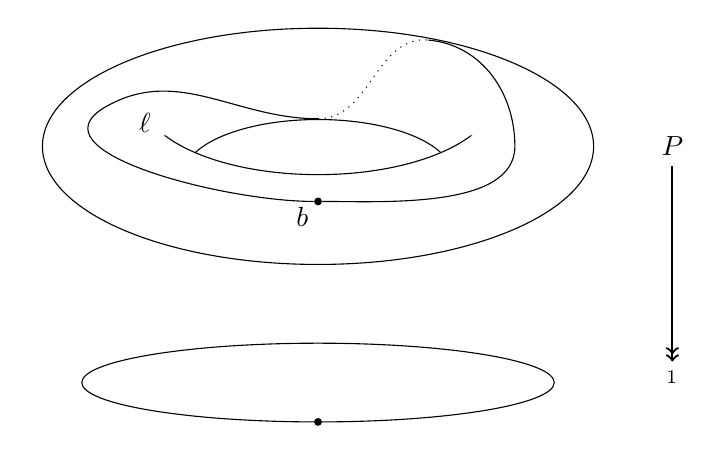
\begin{tikzpicture}
    \draw (0,0) ellipse (3 and .5);
    \draw (0,3) ellipse (3.5 and 1.5);
    \begin{scope}[yshift=4]
      \clip (-3,3) -- (-1.8,3) -- (-1.8,3.7) -- (1.8,3.7) -- (1.8,3) -- (3,3) -- (3,0) -- (-3,0) -- cycle;
      \draw[clip] (0,3.5) ellipse (2.25 and 1);
      \draw (0,2.5) ellipse (1.7 and .7);
    \end{scope}
    \node (P) at (4.5,3) {$P$};
    \node (S1) at (4.5,0) {$\Sn^1$};
    \draw[->>,thick] (P) -- (S1);
    \node[fill,circle,inner sep=1pt,label={below right:$\base$}] at (0,-.5) {};
    \node at (-2.6,.6) {$\lloop$};
    \node[fill,circle,\OPTblue,inner sep=1pt] (b) at (0,2.3) {};
    \node[\OPTblue] at (-.2,2.1) {$b$};
      \begin{scope}
        \draw[\OPTblue] (b) to[out=180,in=-150] (-2.7,3.5) to[out=30,in=180] (0,3.35);
        \draw[\OPTblue,dotted] (0,3.35) to[out=0,in=175] (1.4,4.35);
        \draw[\OPTblue] (1.4,4.35) to[out=-5,in=90] (2.5,3) to[out=-90,in=0,looseness=.8] (b);
      \end{scope}
      \node[\OPTblue] at (-2.2, 3.3) {$\ell$};
  \end{tikzpicture}
  \caption{The topological induction principle for $\Sn^1$}
  \label{fig:topS1ind}
\end{figure}

\begin{figure}
  \centering
  \begin{tikzpicture}
    \draw (0,0) ellipse (3 and .5);
    \draw (0,3) ellipse (3.5 and 1.5);
    \begin{scope}[yshift=4]
      \clip (-3,3) -- (-1.8,3) -- (-1.8,3.7) -- (1.8,3.7) -- (1.8,3) -- (3,3) -- (3,0) -- (-3,0) -- cycle;
      \draw[clip] (0,3.5) ellipse (2.25 and 1);
      \draw (0,2.5) ellipse (1.7 and .7);
    \end{scope}
    \node (P) at (4.5,3) {$P$};
    \node (S1) at (4.5,0) {$\Sn^1$};
    \draw[->>,thick] (P) -- (S1);
    \node[fill,circle,inner sep=1pt,label={below right:$\base$}] at (0,-.5) {};
    \node at (-2.6,.6) {$\lloop$};
    \node[fill,circle,\OPTblue,inner sep=1pt] (b) at (0,2.3) {};
      \node[\OPTblue] at (-.3,2.3) {$b$};
      \node[fill,circle,\OPTpurple,inner sep=1pt] (tb) at (0,1.8) {};
      % \draw[\OPTpurple,dashed] (b) to[out=0,in=0,looseness=5] (0,4) to[out=180,in=180] (tb);
      \draw[\OPTpurple,dashed] (b) arc (-90:90:2.9 and 0.85) arc (90:270:2.8 and 1.1);
      \begin{scope}
        \clip (b) -- ++(.1,0) -- (.1,1.8) -- ++(-.2,0) -- ++(0,-1) -- ++(3,2) -- ++(-3,0) -- (-.1,2.3) -- cycle;
        \draw[\OPTred,dotted,thick] (.2,2.07) ellipse (.2 and .57);
        \begin{scope}
          % \draw[clip] (b) -- ++(.1,0) |- (tb) -- ++(-.2,0) -- ++(0,-1) -| ++(3,3) -| (b);
          \clip (.2,0) rectangle (-2,3);
          \draw[\OPTred,thick] (.2,2.07) ellipse (.2 and .57);
        \end{scope}
      \end{scope}
      \node[\OPTred] at (1,1.2) {$\ell: \trans \lloop b=b$};
  \end{tikzpicture}
  \caption{The type-theoretic induction principle for $\Sn^1$}
  \label{fig:ttS1ind}
\end{figure}

Of course, we expect to be able to prove the recursion principle from the induction principle, by taking $P$ to be a constant type family.
This is in fact the case, although deriving the non-dependent computation rule for $\lloop$ (which refers to $\apfunc f$) from the dependent one (which refers to $\apdfunc f$) is surprisingly a little tricky.

\begin{lem}\label{thm:S1rec}
  \index{recursion principle!for S1@for $\Sn^1$}%
  \index{computation rule!for S1@for $\Sn^1$}%
  If $A$ is a type together with $a:A$ and $p:\id[A]aa$, then there is a
  function $f:\Sn^1\to{}A$ with
  \begin{align*}
    f(\base)&\defeq a \\
    \apfunc f(\lloop)&\defid p.
  \end{align*}
\end{lem}
\begin{proof}
  We would like to apply the induction principle of $\Sn^1$ to the constant type family, $(\lam{x} A): \Sn^1\to \UU$.
  The required hypotheses for this are a point of $(\lam{x} A)(\base) \jdeq A$, which we have (namely $a:A$), and a dependent path in $\dpath {x \mapsto A}{\lloop} a a$, or equivalently $\transfib{x \mapsto A}{\lloop} a = a$.
  This latter type is not the same as the type $\id[A]aa$ where $p$ lives, but it is equivalent to it, because by \autoref{thm:trans-trivial} we have $\transconst{A}{\lloop}{a} : \transfib{x \mapsto A}{\lloop} a= a$.
  Thus, given $a:A$ and $p:a=a$, we can consider the composite
  \[\transconst{A}{\lloop}{a} \ct p:(\dpath {x \mapsto A}\lloop aa).\]
  Applying the induction principle, we obtain $f:\Sn^1\to A$ such that
  \begin{align}
    f(\base) &\jdeq a \qquad\text{and}\label{eq:S1recindbase}\\
    \apdfunc f(\lloop) &= \transconst{A}{\lloop}{a} \ct p.\label{eq:S1recindloop}
  \end{align}
  It remains to derive the equality $\apfunc f(\lloop)=p$.
  However, by \autoref{thm:apd-const}, we have
  \[\apdfunc f(\lloop) = \transconst{A}{\lloop}{f(\base)} \ct \apfunc f(\lloop).\]
  Combining this with~\eqref{eq:S1recindloop} and canceling the occurrences of $\transconstf$ (which are the same by~\eqref{eq:S1recindbase}), we obtain $\apfunc f(\lloop)=p$.
\end{proof}

% Similarly, in this case we speak of defining $f$ by $f(\base)\defeq a$ and $\ap f \lloop \defid p$.
We also have a corresponding uniqueness principle.

\begin{lem}
  \index{uniqueness!principle, propositional!for functions on the circle}%
  If $A$ is a type and $f,g:\Sn^1\to{}A$ are two maps together with two
  equalities $p,q$:
  \begin{align*}
    p:f(\base)&=_Ag(\base),\\
    q:\map{f}\lloop&=^{\lam{x} x=_Ax}_p\map{g}\lloop.
  \end{align*}
  Then for all $x:\Sn^1$ we have $f(x)=g(x)$.
\end{lem}
\begin{proof}
  This is just the induction principle for the type family $P(x)\defeq(f(x)=g(x))$.
\end{proof}

\index{universal!property!of S1@of $\Sn^1$}%
These two lemmas imply the expected universal property of the circle:

\begin{lem}\label{thm:S1ump}
  For any type $A$ we have a natural equivalence
  \[ (\Sn^1 \to A) \;\eqvsym\;
  \sm{x:A} (x=x).
  \]
\end{lem}
\begin{proof}
  We have a canonical function $f:(\Sn^1 \to A) \to \sm{x:A} (x=x)$ defined by $f(g) \defeq (g(\base),\ap g \lloop)$.
  The induction principle shows that the fibers of $f$ are inhabited, while the uniqueness principle shows that they are mere propositions.
  Hence they are contractible, so $f$ is an equivalence.
\end{proof}

\index{type!circle|)}%

As in \autoref{sec:htpy-inductive}, we can show that the conclusion of \autoref{thm:S1ump} is equivalent to having an induction principle with propositional computation rules.
Other higher inductive types also satisfy lemmas analogous to \autoref{thm:S1rec,thm:S1ump}; we will generally leave their proofs to the reader.
We now proceed to consider many examples.


\section{The interval}
\label{sec:interval}

\index{type!interval|(defstyle}%
\indexsee{interval!type}{type, interval}%
The \define{interval}, which we denote $\interval$, is perhaps an even simpler higher inductive type than the circle.
It is generated by:
\begin{itemize}
\item a point $\izero:\interval$,
\item a point $\ione:\interval$, and
\item a path $\seg : \id[\interval]\izero\ione$.
\end{itemize}
\index{recursion principle!for interval type}%
The recursion principle for the interval says that given a type $B$ along with
\begin{itemize}
\item a point $b_0:B$,
\item a point $b_1:B$, and
\item a path $s:b_0=b_1$,
\end{itemize}
there is a function $f:\interval\to B$ such that $f(\izero)\jdeq b_0$, $f(\ione)\jdeq b_1$, and $\ap f \seg = s$.
\index{induction principle!for interval type}%
The induction principle says that given $P:\interval\to\type$ along with
\begin{itemize}
\item a point $b_0:P(\izero)$,
\item a point $b_1:P(\ione)$, and
\item a path $s:\dpath{P}{\seg}{b_0}{b_1}$,
\end{itemize}
there is a function $f:\prd{x:\interval} P(x)$ such that $f(\izero)\jdeq b_0$, $f(\ione)\jdeq b_1$, and $\apd f \seg = s$.

Regarded purely up to homotopy, the interval is not really interesting:

\begin{lem}
  The type $\interval$ is contractible.
\end{lem}

\begin{proof}
  We prove that for all $x:\interval$ we have $x=_\interval\ione$. In other words we want a
  function $f$ of type $\prd{x:\interval}(x=_\interval\ione)$. We begin to define $f$ in the following way:
  \begin{alignat*}{2}
    f(\izero)&\defeq \seg  &:\izero&=_\interval\ione,\\
    f(\ione)&\defeq \refl\ione &:\ione &=_\interval\ione.
  \end{alignat*}
  It remains to define $\apd{f}\seg$, which must have type $\seg =_\seg^{\lam{x} x=_\interval\ione}\refl \ione$.
  By definition this type is $\trans\seg\seg=_{\ione=_\interval\ione}\refl\ione$, which in turn is equivalent to $\rev\seg\ct\seg=\refl\ione$.
  But there is a canonical element of that type, namely the proof that path inverses are in fact inverses.
\end{proof}

However, type-theoretically the interval does still have some interesting features, just like the topological interval in classical homotopy theory.
For instance, it enables us to give an easy proof of function extensionality.
(Of course, as in \autoref{sec:univalence-implies-funext}, for the duration of the following proof we suspend our overall assumption of the function extensionality axiom.)

\begin{lem}\label{thm:interval-funext}
  \index{function extensionality!proof from interval type}%
  If $f,g:A\to{}B$ are two functions such that $f(x)=g(x)$ for every $x:A$, then
  $f=g$ in the type $A\to{}B$.
\end{lem}

\begin{proof}
  Let's call the proof we have $p:\prd{x:A}(f(x)=g(x))$. For all $x:A$ we define
  a function $\widetilde{p}_x:\interval\to{}B$ by
  \begin{align*}
    \widetilde{p}_x(\izero) &\defeq f(x), \\
    \widetilde{p}_x(\ione) &\defeq g(x), \\
    \map{\widetilde{p}_x}\seg &\defid p(x).
  \end{align*}
  We now define $q:\interval\to(A\to{}B)$ by
  \[q(i)\defeq(\lam{x} \widetilde{p}_x(i))\]
  Then $q(\izero)$ is the function $\lam{x} \widetilde{p}_x(\izero)$, which is equal to $f$ because $\widetilde{p}_x(\izero)$ is defined by $f(x)$.
  Similarly, we have $q(\ione)=g$, and hence
  \[\map{q}\seg:f=_{(A\to{}B)}g \qedhere\]
\end{proof}

\index{type!interval|)}%

\section{Circles and spheres}
\label{sec:circle}

\index{type!circle|(}%
We have already discussed the circle $\Sn^1$ as the higher inductive type generated by
\begin{itemize}
\item A point $\base:\Sn^1$, and
\item A path $\lloop : {\id[\Sn^1]\base\base}$.
\end{itemize}
\index{induction principle!for S1@for $\Sn^1$}%
Its induction principle says that given $P:\Sn^1\to\type$ along with $b:P(\base)$ and $\ell :\dpath P \lloop b b$, we have $f:\prd{x:\Sn^1} P(x)$ with $f(\base)\jdeq b$ and $\apd f \lloop = \ell$.
Its non-dependent recursion principle says that given $B$ with $b:B$ and $\ell:b=b$, we have $f:\Sn^1\to B$ with $f(\base)\jdeq b$ and $\ap f \lloop = \ell$.

We observe that the circle is nontrivial.

\begin{lem}\label{thm:loop-nontrivial}
  $\lloop\neq\refl{\base}$.
\end{lem}
\begin{proof}
  Suppose that $\lloop=\refl{\base}$.
  Then since for any type $A$ with $x:A$ and $p:x=x$, there is a function $f:\Sn^1\to A$ defined by $f(\base)\defeq x$ and $\ap f \lloop \defid p$, we have
  \[p = f(\lloop) = f(\refl{\base}) = \refl{x}.\]
  But this implies that every type is a set, which as we have seen is not the case (see \autoref{thm:type-is-not-a-set}).
\end{proof}

The circle also has the following interesting property, which is useful as a source of counterexamples.

\begin{lem}\label{thm:S1-autohtpy}
  There exists an element of $\prd{x:\Sn^1} (x=x)$ which is not equal to $x\mapsto \refl{x}$.
\end{lem}
\begin{proof}
  We define $f:\prd{x:\Sn^1} (x=x)$ by $\Sn^1$-induction.
  When $x$ is $\base$, we let $f(\base)\defeq \lloop$.
  Now when $x$ varies along $\lloop$ (see \autoref{rmk:varies-along}), we must show that $\transfib{x\mapsto x=x}{\lloop}{\lloop} = \lloop$.
  However, in \autoref{sec:compute-paths} we observed that $\transfib{x\mapsto x=x}{p}{q} = \opp{p} \ct q \ct p$, so what we have to show is that $\opp{\lloop} \ct \lloop \ct \lloop = \lloop$.
  But this is clear by canceling an inverse.

  To show that $f\neq (x\mapsto \refl{x})$, it suffices by function extensionality to show that $f(\base) \neq \refl{\base}$.
  But $f(\base)=\lloop$, so this is just the previous lemma.
\end{proof}

For instance, this enables us to extend \autoref{thm:type-is-not-a-set} by showing that any universe which contains the circle cannot be a 1-type.

\begin{cor}
  If the type $\Sn^1$ belongs to some universe \type, then \type is not a 1-type.
\end{cor}
\begin{proof}
  The type $\Sn^1=\Sn^1$ in \type is, by univalence, equivalent to the type $\eqv{\Sn^1}{\Sn^1}$ of auto\-equivalences of $\Sn^1$, so it suffices to show that $\eqv{\Sn^1}{\Sn^1}$ is not a set.
  \index{automorphism!of S1@of $\Sn^1$}%
  For this, it suffices to show that its equality type $\id[(\eqv{\Sn^1}{\Sn^1})]{\idfunc[\Sn^1]}{\idfunc[\Sn^1]}$ is not a mere proposition.
  Since being an equivalence is a mere proposition, this type is equivalent to $\id[(\Sn^1\to\Sn^1)]{\idfunc[\Sn^1]}{\idfunc[\Sn^1]}$.
  But by function extensionality, this is equivalent to $\prd{x:\Sn^1} (x=x)$, which as we have seen in \autoref{thm:S1-autohtpy} contains two unequal elements.
\end{proof}

\index{type!circle|)}%

\index{type!2-sphere|(}%
\indexsee{sphere type}{type, sphere}%
We have also mentioned that the 2-sphere $\Sn^2$ should be the higher inductive type generated by
\symlabel{s2b}
\begin{itemize}
\item A point $\base:\Sn^2$, and
\item A 2-dimensional path $\surf:\refl{\base} = \refl{\base}$ in ${\base=\base}$.
\end{itemize}
\index{recursion principle!for S2@for $\Sn^2$}%
The recursion principle for $\Sn^2$ is not hard: it says that given $B$ with $b:B$ and $s:\refl b = \refl b$, we have $f:\Sn^2\to B$ with $f(\base)\jdeq b$ and $\aptwo f \surf = s$.
Here by ``$\aptwo f \surf$'' we mean an extension of the functorial action of $f$ to two-dimensional paths, which can be stated precisely as follows.

\begin{lem}\label{thm:ap2}
  Given $f:A\to B$ and $x,y:A$ and $p,q:x=y$, and $r:p=q$, we have a path $\aptwo f r : \ap f p = \ap f q$.
\end{lem}
\begin{proof}
  By path induction, we may assume $p\jdeq q$ and $r$ is reflexivity.
  But then we may define $\aptwo f {\refl p} \defeq \refl{\ap f p}$.
\end{proof}

In order to state the general induction principle, we need a version of this lemma for dependent functions, which in turn requires a notion of dependent two-dimensional paths.
As before, there are many ways to define such a thing; one is by way of a two-dimensional version of transport.

\begin{lem}\label{thm:transport2}
  Given $P:A\to\type$ and $x,y:A$ and $p,q:x=y$ and $r:p=q$, for any $u:P(x)$ we have $\transtwo r u : \trans p u = \trans q u$.
\end{lem}
\begin{proof}
  By path induction.
\end{proof}

Now suppose given $x,y:A$ and $p,q:x=y$ and $r:p=q$ and also points $u:P(x)$ and $v:P(y)$ and dependent paths $h:\dpath P p u v$ and $k:\dpath P q u v$.
By our definition of dependent paths, this means $h:\trans p u = v$ and $k:\trans q u = v$.
Thus, it is reasonable to define the type of dependent 2-paths over $r$ to be
\[ (\dpath P r h k )\defeq (h = \transtwo r u \ct k). \]
We can now state the dependent version of \autoref{thm:ap2}.

\begin{lem}\label{thm:apd2}
  Given $P:A\to\type$ and $x,y:A$ and $p,q:x=y$ and $r:p=q$ and a function $f:\prd{x:A} P(x)$, we have
  $\apdtwo f r : \dpath P r {\apd f p}{\apd f q}$.
\end{lem}
\begin{proof}
  Path induction.
\end{proof}

\index{induction principle!for S2@for $\Sn^2$}%
Now we can state the induction principle for $\Sn^2$: given $P:\Sn^2\to P$ with $b:P(\base)$ and $s:\dpath P \surf {\refl b}{\refl b}$, there is a function $f:\prd{x:\Sn^2} P(x)$ such that $f(\base)\jdeq b$ and $\apdtwo f \surf = s$.

\index{type!2-sphere|)}%

Of course, this explicit approach gets more and more complicated as we go up in dimension.
Thus, if we want to define $n$-spheres for all $n$, we need some more systematic idea.
One approach is to work with $n$-dimensional loops\index{loop!n-@$n$-} directly, rather than general $n$-dimensional paths.\index{path!n-@$n$-}

\index{type!pointed}%
Recall from \autoref{sec:equality} the definitions of \emph{pointed types} $\type_*$, and the $n$-fold loop space\index{loop space!iterated} $\Omega^n : \type_* \to \type_*$
(\cref{def:pointedtype,def:loopspace}).  Now we can define the
$n$-sphere $\Sn^n$ to be the higher inductive type generated by
\index{type!n-sphere@$n$-sphere}%
\begin{itemize}
\item A point $\base:\Sn^n$, and
\item An $n$-loop $\lloop_n : \Omega^n(\Sn^n,\base)$.
\end{itemize}
In order to write down the induction principle for this presentation, we would need to define a notion of ``dependent $n$-loop\indexdef{loop!dependent n-@dependent $n$-}'', along with the action of dependent functions on $n$-loops.
We leave this to the reader (see \autoref{ex:nspheres}); in the next section we will discuss a different way to define the spheres that is sometimes more tractable.


\section{Suspensions}
\label{sec:suspension}

\indexsee{type!suspension of}{suspension}%
\index{suspension|(defstyle}%
The \define{suspension} of a type $A$ is the universal way of making the points of $A$ into paths (and hence the paths in $A$ into 2-paths, and so on).
It is a type $\susp A$ defined by the following generators:\footnote{There is an unfortunate clash of notation with dependent pair types, which of course are also written with a $\Sigma$.
  However, context usually disambiguates.}
\begin{itemize}
\item a point $\north:\susp A$,
\item a point $\south:\susp A$, and
\item a function $\merid:A \to (\id[\susp A]\north\south)$.
\end{itemize}
The names are intended to suggest a ``globe'' of sorts, with a north pole, a south pole, and an $A$'s worth of meridians
\indexdef{pole}%
\indexdef{meridian}%
from one to the other.
Indeed, as we will see, if $A=\Sn^1$, then its suspension is equivalent to the surface of an ordinary sphere, $\Sn^2$.

\index{recursion principle!for suspension}%
The recursion principle for $\susp A$ says that given a type $B$ together with
\begin{itemize}
\item points $n,s:B$ and
\item a function $m:A \to (n=s)$,
\end{itemize}
we have a function $f:\susp A \to B$ such that $f(\north)\jdeq n$ and $f(\south)\jdeq s$, and for all $a:A$ we have $\ap f {\merid(a)} = m(a)$.
\index{induction principle!for suspension}%
Similarly, the induction principle says that given $P:\susp A \to \type$ together with
\begin{itemize}
\item a point $n:P(\north)$,
\item a point $s:P(\south)$, and
\item for each $a:A$, a path $m(a):\dpath P{\merid(a)}ns$,
\end{itemize}
there exists a function $f:\prd{x:\susp A} P(x)$ such that $f(\north)\jdeq n$ and $f(\south)\jdeq s$ and for each $a:A$ we have $\apd f {\merid(a)} = m(a)$.

Our first observation about suspension is that it gives another way to define the circle.

\begin{lem}\label{thm:suspbool}
  \index{type!circle}%
  $\eqv{\susp\bool}{\Sn^1}$.
\end{lem}
\begin{proof}
  Define $f:\susp\bool\to\Sn^1$ by recursion such that $f(\north)\defeq \base$ and $f(\south)\defeq\base$, while $\ap f{\merid(\bfalse)}\defid\lloop$ but $\ap f{\merid(\btrue)} \defid \refl{\base}$.
  Define $g:\Sn^1\to\susp\bool$ by recursion such that $g(\base)\defeq \north$ and $\ap g \lloop \defid \merid(\bfalse) \ct \opp{\merid(\btrue)}$.
  We now show that $f$ and $g$ are quasi-inverses.

  First we show by induction that $g(f(x))=x$ for all $x:\susp \bool$.
  If $x\jdeq\north$, then $g(f(\north)) \jdeq g(\base)\jdeq \north$, so we have $\refl{\north} : g(f(\north))=\north$.
  If $x\jdeq\south$, then $g(f(\south)) \jdeq g(\base)\jdeq \north$, and we choose the equality $\merid(\btrue) : g(f(\south)) = \south$.
  It remains to show that for any $y:\bool$, these equalities are preserved as $x$ varies along $\merid(y)$, which is to say that when $\refl{\north}$ is transported along $\merid(y)$ it yields $\merid(\btrue)$.
  By transport in path spaces and pulled back fibrations, this means we are to show that
  \[ \opp{\ap g {\ap f {\merid(y)}}} \ct \refl{\north} \ct \merid(y) = \merid(\btrue). \]
  Of course, we may cancel $\refl{\north}$.
  Now by \bool-induction, we may assume either $y\jdeq \bfalse$ or $y\jdeq \btrue$.
  If $y\jdeq \bfalse$, then we have
  \begin{align*}
    \opp{\ap g {\ap f {\merid(\bfalse)}}} \ct \merid(\bfalse)
    &= \opp{\ap g {\lloop}} \ct \merid(\bfalse)\\
    &= \opp{(\merid(\bfalse) \ct \opp{\merid(\btrue)})} \ct \merid(\bfalse)\\
    &= \merid(\btrue) \ct \opp{\merid(\bfalse)} \ct \merid(\bfalse)\\
    &= \merid(\btrue)
  \end{align*}
  while if $y\jdeq \btrue$, then we have
  \begin{align*}
    \opp{\ap g {\ap f {\merid(\btrue)}}} \ct \merid(\btrue)
    &= \opp{\ap g {\refl{\base}}} \ct \merid(\btrue)\\
    &= \opp{\refl{\north}} \ct \merid(\btrue)\\
    &= \merid(\btrue).
  \end{align*}
  Thus, for all $x:\susp \bool$, we have $g(f(x))=x$.

  Now we show by induction that $f(g(x))=x$ for all $x:\Sn^1$.
  If $x\jdeq \base$, then $f(g(\base))\jdeq f(\north)\jdeq\base$, so we have $\refl{\base} : f(g(\base))=\base$.
  It remains to show that this equality is preserved as $x$ varies along $\lloop$, which is to say that it is transported along $\lloop$ to itself.
  Again, by transport in path spaces and pulled back fibrations, this means to show that
  \[ \opp{\ap f {\ap g {\lloop}}} \ct \refl{\base} \ct \lloop = \refl{\base}.\]
  However, we have
  \begin{align*}
    \ap f {\ap g {\lloop}} &= \ap f {\merid(\bfalse) \ct \opp{\merid(\btrue)}}\\
    &= \ap f {\merid(\bfalse)} \ct \opp{\ap f {\merid(\btrue)}}\\
    &= \lloop \ct \refl{\base}
  \end{align*}
  so this follows easily.
\end{proof}

Topologically, the two-point space \bool is also known as the \emph{0-dimensional sphere}, $\Sn^0$.
(For instance, it is the space of points at distance $1$ from the origin in $\mathbb{R}^1$, just as the topological 1-sphere is the space of points at distance $1$ from the origin in $\mathbb{R}^2$.)
Thus, \autoref{thm:suspbool} can be phrased suggestively as $\eqv{\susp\Sn^0}{\Sn^1}$.
\index{type!n-sphere@$n$-sphere|defstyle}%
\indexsee{n-sphere@$n$-sphere}{type, $n$-sphere}%
In fact, this pattern continues: we can define all the spheres inductively by
\begin{equation}\label{eq:Snsusp}
  \Sn^0 \defeq \bool
  \qquad\text{and}\qquad
  \Sn^{n+1} \defeq \susp \Sn^n.
\end{equation}
We can even start one dimension lower by defining $\Sn^{-1}\defeq \emptyt$, and observe that $\eqv{\susp\emptyt}{\bool}$.

To prove carefully that this agrees with the definition of $\Sn^n$ from the previous section would require making the latter more explicit.
However, we can show that the recursive definition has the same universal property that we would expect the other one to have.
If $(A,a_0)$ and $(B,b_0)$ are pointed types (with basepoints often left implicit), let $\Map_*(A,B)$ denote the type of based maps:
\index{based map}
\symlabel{based-maps}
\[ \Map_*(A,B) \defeq \sm{f:A\to B} (f(a_0)=b_0). \]
Note that any type $A$ gives rise to a pointed type $A_+ \defeq A+\unit$ with basepoint $\inr(\ttt)$; this is called \emph{adjoining a disjoint basepoint}.
\indexdef{basepoint!adjoining a disjoint}%
\index{disjoint!basepoint}%
\index{adjoining a disjoint basepoint}%

\begin{lem}
  For a type $A$ and a pointed type $(B,b_0)$, we have
  \[ \eqv{\Map_*(A_+,B)}{(A\to B)} \]
\end{lem}
Note that on the right we have the ordinary type of \emph{unbased} functions from $A$ to $B$.
\begin{proof}
  From left to right, given $f:A_+ \to B$ with $p:f(\inr(\ttt)) = b_0$, we have $f\circ \inl : A \to B$.
  And from right to left, given $g:A\to B$ we define $g':A_+ \to B$ by $g'(\inl(a))\defeq g(a)$ and $g'(\inr(u)) \defeq b_0$.
  We leave it to the reader to show that these are quasi-inverse operations.
\end{proof}

In particular, note that $\eqv{\bool}{\unit_+}$.
Thus, for any pointed type $B$ we have
\[{\Map_*(\bool,B)} \eqvsym {(\unit \to B)}\eqvsym B.\]
%
Now recall that the loop space\index{loop space} operation $\Omega$ acts on pointed types, with definition $\Omega(A,a_0) \defeq (\id[A]{a_0}{a_0},\refl{a_0})$.
We can also make the suspension $\susp$ act on pointed types, by $\susp(A,a_0)\defeq (\susp A,\north)$.

\begin{lem}\label{lem:susp-loop-adj}
  \index{universal!property!of suspension}%
  For pointed types $(A,a_0)$ and $(B,b_0)$ we have
  \[ \eqv{\Map_*(\susp A, B)}{\Map_*(A,\Omega B)}.\]
\end{lem}
\begin{proof}
  From left to right, given $f:\susp A \to B$ with $p:f(\north) = b_0$, we define $g:A \to \Omega B$ by
  \[g(a) \defeq \opp p \ct \ap f{\merid(a) \ct \opp{\merid(a_0)}} \ct p.\]
  Then we have
  \begin{align*}
    g(a_0) &\jdeq \opp p \ct \ap f{\merid(a_0) \ct \opp{\merid(a_0)}} \ct p\\
    &= \opp p \ct \ap f{\refl{\north}} \ct p\\
    &= \opp p \ct p\\
    &= \refl{b_0}.
  \end{align*}
  Thus, denoting this path by $q:g(a_0)=\refl{b_0}$, we have $(g,q):\Map_*(A,\Omega B)$.

  On the other hand, from right to left, given $g:A\to \Omega B$ and $q:g(a_0)=\refl{b_0}$, we define $f:\susp A \to B$ by $\susp$-recursion, such that $f(\north)\defeq b_0$ and $f(\south)\defeq b_0$ and
  \[ \ap f {\merid(a)} \defid g(a). \]
  Then we can simply take $p$ to be $\refl{b_0} : f(\north)= b_0$.

  Now given $(f,p)$, by passing back and forth we obtain $(f',p')$ where $f'$ is defined by $f'(\north)\jdeq b_0$ and $f'(\south)\jdeq b_0$ and
  \[ \ap {f'} {\merid(a)} = \opp p \ct \ap f{\merid(a) \ct \opp{\merid(a_0)}} \ct p, \]
  while $p' \jdeq \refl{b_0}$.
  To show $f=f'$, by function extensionality it suffices to show $f(x)=f'(x)$ for all $x:\susp A$, so we can use the induction principle of suspension.
  First, we have
  \begin{equation}
    f(\north) \overset{p}{=} b_0 \jdeq f'(\north). \label{eq:ffprime-north}
  \end{equation}
  Second, we have
  \[\xymatrix@C=4pc{ f(\south) \ar@{=}[r]^-{\opp{\ap f {\merid(a_0)}}} & f(\north) \overset{\smash p}{=} b_0 \jdeq f'(\south).}\]
  And thirdly, as $x$ varies along $\merid(a)$ we must show that the following diagram of paths commutes (invoking the definition of $\ap{f'}{\merid(a)}$):
  \[ \xymatrix{
    f(\north) \ar@{=}[rrr]^-{p} \ar@{=}[ddd]_{f(\merid(a))} &&&
    b_0 \ar@{=}[r]^-{\refl{}} &
    f'(\north) \ar@{=}[d]^{\opp p}\\
    &&&& f(\north) \ar@{=}[d]^{\ap f{\merid(a) \ct \opp{\merid(a_0)}}}\\
    &&&& f(\north) \ar@{=}[d]^p\\
    f(\south) \ar@{=}[rr]_-{\opp{\ap f {\merid(a_0)}}} &&
    f(\north) \ar@{=}[r]_-p &
    b_0 \ar@{=}[r]_-{\refl{}} &
    f'(\south) }
  \]
  This is clear.
  Thus, to show that $(f,p)=(f',p')$, it remains only to show that $p$ is identified with $p'$ when transported along this equality $f=f'$.
  Since the type of $p$ is $f(\north)=b_0$, this means essentially that when $p$ is composed on the left with the inverse of the equality~\eqref{eq:ffprime-north}, it becomes $p'$.
  But this is obvious, since~\eqref{eq:ffprime-north} is just $p$ itself, while $p'$ is reflexivity.

  On the other side, suppose given $(g,q)$.
  By passing back and forth we obtain $(g',q')$ with
  \begin{align*}
    g'(a) &= \opp{\refl{b_0}} \ct g(a) \ct \opp{g(a_0)} \ct \refl{b_0}\\
    &= g(a) \ct \opp{g(a_0)}\\
    &= g(a)
  \end{align*}
  using $q:g(a_0) = \refl{b_0}$ in the last equality.
  Thus, $g'=g$ by function extensionality, so it remains to show that when transported along this equality $q$ is identified with $q'$.
  At $a_0$, the induced equality $g(a_0)=g'(a_0)$ consists essentially of $q$ itself, while the definition of $q'$ involves only canceling inverses and reflexivities.
  Thus, some tedious manipulations of naturality finish the proof.
\end{proof}

\index{type!n-sphere@$n$-sphere|defstyle}%
In particular, for the spheres defined as in~\eqref{eq:Snsusp} we have
\index{universal!property!of Sn@of $\Sn^n$}%
\[ \Map_*(\Sn^n,B) \eqvsym \Map_*(\Sn^{n-1}, \Omega B) \eqvsym \cdots \eqvsym \Map_*(\bool,\Omega^n B) \eqvsym \Omega^n B. \]
Thus, these spheres $\Sn^n$ have the universal property that we would expect from the spheres defined directly in terms of $n$-fold loop spaces\index{loop space!iterated} as in \autoref{sec:circle}.

\index{suspension|)}%

\section{Cell complexes}
\label{sec:cell-complexes}

\index{cell complex|(defstyle}%
\index{CW complex|(defstyle}%
In classical topology, a \emph{cell complex} is a space obtained by successively attaching discs along their boundaries.
It is called a \emph{CW complex} if the boundary of an $n$-dimensional disc\index{disc} is constrained to lie in the discs of dimension strictly less than $n$ (the $(n-1)$-skeleton).\index{skeleton!of a CW-complex}

Any finite CW complex can be presented as a higher inductive type, by turning $n$-dimensional discs into $n$-dimensional paths and partitioning the image of the attaching\index{attaching map} map into a source\index{source!of a path constructor} and a target\index{target!of a path constructor}, with each written as a composite of lower dimensional paths.
Our explicit definitions of $\Sn^1$ and $\Sn^2$ in \autoref{sec:circle} had this form.

\index{torus}%
Another example is the torus $T^2$, which is generated by:
\begin{itemize}
\item a point $b:T^2$,
\item a path $p:b=b$,
\item another path $q:b=b$, and
\item a 2-path $t: p\ct q = q \ct p$.
\end{itemize}
Perhaps the easiest way to see that this is a torus is to start with a rectangle, having four corners $a,b,c,d$, four edges $p,q,r,s$, and an interior which is manifestly a 2-path $t$ from $p\ct q$ to $r\ct s$:
\begin{equation*}
  \xymatrix{
      a\ar@{=}[r]^p\ar@{=}[d]_r \ar@{}[dr]|{\Downarrow t} &
      b\ar@{=}[d]^q\\
      c\ar@{=}[r]_s &
      d
      }
\end{equation*}
Now identify the edge $r$ with $q$ and the edge $s$ with $p$, resulting in also identifying all four corners.
Topologically, this identification can be seen to produce a torus.

\index{induction principle!for torus}%
\index{torus!induction principle for}%
The induction principle for the torus is the trickiest of any we've written out so far.
Given $P:T^2\to\type$, for a section $\prd{x:T^2} P(x)$ we require
\begin{itemize}
\item a point $b':P(b)$,
\item a path $p' : \dpath P p {b'} {b'}$,
\item a path $q' : \dpath P q {b'} {b'}$, and
\item a 2-path $t'$ between the ``composites'' $p'\ct q'$ and $q'\ct p'$, lying over $t$.
\end{itemize}
In order to make sense of this last datum, we need a composition operation for dependent paths, but this is not hard to define.
Then the induction principle gives a function $f:\prd{x:T^2} P(x)$ such that $f(b)\jdeq b'$ and $\apd f {p} = p'$ and $\apd f {q} = q'$ and something like ``$\apdtwo f t = t'$''.
However, this is not well-typed as it stands, firstly because the equalities $\apd f {p} = p'$ and $\apd f {q} = q'$ are not judgmental, and secondly because $\apdfunc f$ only preserves path concatenation up to homotopy.
We leave the details to the reader (see \autoref{ex:torus}).

Of course, another definition of the torus is $T^2 \defeq \Sn^1 \times \Sn^1$ (in \autoref{ex:torus-s1-times-s1} we ask the reader to verify the equivalence of the two).
\index{Klein bottle}%
\index{projective plane}%
The cell-complex definition, however, generalizes easily to other spaces without such descriptions, such as the Klein bottle, the projective plane, etc.
But it does get increasingly difficult to write down the induction principles, requiring us to define notions of dependent $n$-paths and of $\apdfunc{}$ acting on $n$-paths.
Fortunately, once we have the spheres in hand, there is a way around this.

\section{Hubs and spokes}
\label{sec:hubs-spokes}

\indexsee{spoke}{hub and spoke}%
\index{hub and spoke|(defstyle}%

In topology, one usually speaks of building CW complexes by attaching $n$-dimensional discs along their $(n-1)$-dimensional boundary spheres.
\index{attaching map}%
However, another way to express this is by gluing in the \emph{cone}\index{cone!of a sphere} on an $(n-1)$-dimensional sphere.
That is, we regard a disc\index{disc} as consisting of a cone point (or ``hub''), with meridians
\index{meridian}%
(or ``spokes'') connecting that point to every point on the boundary, continuously, as shown in \autoref{fig:hub-and-spokes}.

\begin{figure}
  \centering
  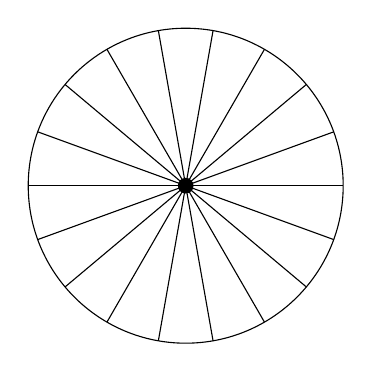
\begin{tikzpicture}
    \draw (0,0) circle (2cm);
    \foreach \x in {0,20,...,350}
      \draw[\OPTblue] (0,0) -- (\x:2cm);
    \node[\OPTblue,circle,fill,inner sep=2pt] (hub) at (0,0) {};
  \end{tikzpicture}
  \caption{A 2-disc made out of a hub and spokes}
  \label{fig:hub-and-spokes}
\end{figure}

We can use this idea to express higher inductive types containing $n$-dimensional path-con\-struc\-tors for $n>1$ in terms of ones containing only 1-di\-men\-sion\-al path-con\-struc\-tors.
The point is that we can obtain an $n$-dimensional path as a continuous family of 1-dimensional paths parametrized by an $(n-1)$-di\-men\-sion\-al object.
The simplest $(n-1)$-dimensional object to use is the $(n-1)$-sphere, although in some cases a different one may be preferable.
(Recall that we were able to define the spheres in \autoref{sec:suspension} inductively using suspensions, which involve only 1-dimensional path constructors.
Indeed, suspension can also be regarded as an instance of this idea, since it involves a family of 1-dimensional paths parametrized by the type being suspended.)

\index{torus}
For instance, the torus $T^2$ from the previous section could be defined instead to be generated by:
\begin{itemize}
\item a point $b:T^2$,
\item a path $p:b=b$,
\item another path $q:b=b$,
\item a point $h:T^2$, and
\item for each $x:\Sn^1$, a path $s(x) : f(x)=h$, where $f:\Sn^1\to T^2$ is defined by $f(\base)\defeq b$ and $\ap f \lloop \defid p \ct q \ct \opp p \ct \opp q$.
\end{itemize}
The induction principle for this version of the torus says that given $P:T^2\to\type$, for a section $\prd{x:T^2} P(x)$ we require
\begin{itemize}
\item a point $b':P(b)$,
\item a path $p' : \dpath P p {b'} {b'}$,
\item a path $q' : \dpath P q {b'} {b'}$,
\item a point $h':P(h)$, and
\item for each $x:\Sn^1$, a path $\dpath {P}{s(x)}{g(x)}{h'}$, where $g:\prd{x:\Sn^1} P(f(x))$ is defined by $g(\base)\defeq b'$ and $\apd g \lloop \defid p' \ct q' \ct \opp{(p')} \ct \opp{(q')}$.
\end{itemize}
Note that there is no need for dependent 2-paths or $\apdtwofunc{}$.
We leave it to the reader to write out the computation rules.

\begin{rmk}\label{rmk:spokes-no-hub}
One might question the need for introducing the hub point $h$; why couldn't we instead simply add paths continuously relating the boundary of the disc to a point \emph{on} that boundary, as shown in \autoref{fig:spokes-no-hub}?
This does work, but not as well.
For if, given some $f:\Sn^1 \to X$, we give a path constructor connecting each $f(x)$ to $f(\base)$, then what we end up with is more like the picture in \autoref{fig:spokes-no-hub-ii} of a cone whose vertex is twisted around and glued to some point on its base.
The problem is that the specified path from $f(\base)$ to itself may not be reflexivity.
We could add a 2-dimensional path constructor ensuring this, but using a separate hub avoids the need for any path constructors of dimension above~$1$.
\end{rmk}

\begin{figure}
  \centering
  \begin{minipage}{2in}
    \begin{center}
      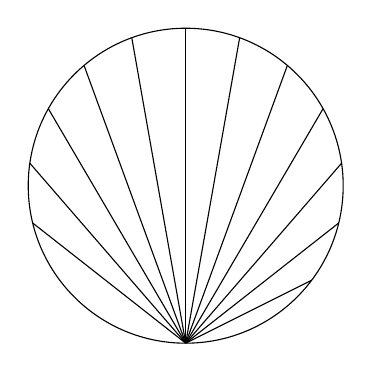
\begin{tikzpicture}
        \draw (0,0) circle (2cm);
        \clip (0,0) circle (2cm);
        \foreach \x in {0,15,...,165}
        \draw[\OPTblue] (0,-2cm) -- (\x:4cm);
      \end{tikzpicture}
    \end{center}
    \caption{Hubless spokes}
    \label{fig:spokes-no-hub}
  \end{minipage}
  \qquad
  \begin{minipage}{2in}
    \begin{center}
      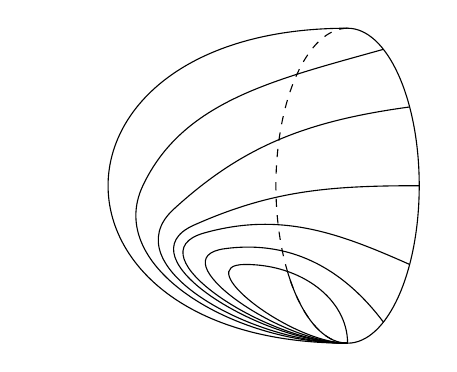
\begin{tikzpicture}[xscale=1.3]
        \draw (0,0) arc (-90:90:.7cm and 2cm) ;
        \draw[dashed] (0,4cm) arc (90:270:.7cm and 2cm) ;
        \draw[\OPTblue] (0,0) to[out=90,in=0] (-1,1) to[out=180,in=180] (0,0);
        \draw[\OPTblue] (0,4cm) to[out=180,in=180,looseness=2] (0,0);
        \path (0,0) arc (-90:-60:.7cm and 2cm) node (a) {};
        \draw[\OPTblue] (a.center) to[out=120,in=10] (-1.2,1.2) to[out=190,in=180] (0,0);
        \path (0,0) arc (-90:-30:.7cm and 2cm) node (b) {};
        \draw[\OPTblue] (b.center) to[out=150,in=20] (-1.4,1.4) to[out=200,in=180] (0,0);
        \path (0,0) arc (-90:0:.7cm and 2cm) node (c) {};
        \draw[\OPTblue] (c.center) to[out=180,in=30] (-1.5,1.5) to[out=210,in=180] (0,0);
        \path (0,0) arc (-90:30:.7cm and 2cm) node (d) {};
        \draw[\OPTblue] (d.center) to[out=190,in=50] (-1.7,1.7) to[out=230,in=180] (0,0);
        \path (0,0) arc (-90:60:.7cm and 2cm) node (e) {};
        \draw[\OPTblue] (e.center) to[out=200,in=70] (-2,2) to[out=250,in=180] (0,0);
        \clip (0,0) to[out=90,in=0] (-1,1) to[out=180,in=180] (0,0);
        \draw (0,4cm) arc (90:270:.7cm and 2cm) ;
      \end{tikzpicture}
    \end{center}
    \caption{Hubless spokes, II}
    \label{fig:spokes-no-hub-ii}
  \end{minipage}
\end{figure}

\begin{rmk}
  \index{computation rule!propositional}%
  Note also that this ``translation'' of higher paths into 1-paths does not preserve judgmental computation rules for these paths, though it does preserve propositional ones.
\end{rmk}

\index{cell complex|)}%
\index{CW complex|)}%

\index{hub and spoke|)}%


\section{Pushouts}
\label{sec:colimits}

\index{type!limit}%
\index{type!colimit}%
\index{limit!of types}%
\index{colimit!of types}%
From a category-theoretic point of view, one of the important aspects of any foundational system is the ability to construct limits and colimits.
In set-theoretic foundations, these are limits and colimits of sets, whereas in our case they are limits and colimits of \emph{types}.
We have seen in \autoref{sec:universal-properties} that cartesian product types have the correct universal property of a categorical product of types, and in \autoref{ex:coprod-ump} that coproduct types likewise have their expected universal property.

As remarked in \autoref{sec:universal-properties}, more general limits can be constructed using identity types and $\Sigma$-types, e.g.\ the pullback\index{pullback} of $f:A\to C$ and $g:B\to C$ is $\sm{a:A}{b:B} (f(a)=g(b))$ (see \autoref{ex:pullback}).
However, more general \emph{colimits} require identifying elements coming from different types, for which higher inductives are well-adapted.
Since all our constructions are homotopy-invariant, all our colimits are necessarily \emph{homotopy colimits}, but we drop the ubiquitous adjective in the interests of concision.

In this section we discuss \emph{pushouts}, as perhaps the simplest and one of the most useful colimits.
Indeed, one expects all finite colimits (for a suitable homotopical definition of ``finite'') to be constructible from pushouts and finite coproducts.
It is also possible to give a direct construction of more general colimits using higher inductive types, but this is somewhat technical, and also not completely satisfactory since we do not yet have a good fully general notion of homotopy coherent diagrams.

\indexsee{type!pushout of}{pushout}%
\index{pushout|(defstyle}%
\index{span}%
Suppose given a span of types and functions:
\[\Ddiag=\;\vcenter{\xymatrix{C \ar^g[r] \ar_f[d] & B \\ A & }}\]
The \define{pushout} of this span is the higher inductive type $A\sqcup^CB$ presented by
\begin{itemize}
\item a function $\inl:A\to A\sqcup^CB$,
\item a function $\inr:B \to A\sqcup^CB$, and
\item for each $c:C$ a path $\glue(c):(\inl(f(c))=\inr(g(c)))$.
\end{itemize}
In other words, $A\sqcup^CB$ is the disjoint union of $A$ and $B$, together with for every $c:C$ a witness that $f(c)$ and $g(c)$ are equal.
The recursion principle says that if $D$ is another type, we can define a map $s:A\sqcup^CB\to{}D$ by defining
\begin{itemize}
\item for each $a:A$, the value of $s(\inl(a)):D$,
\item for each $b:B$, the value of $s(\inr(b)):D$, and
\item for each $c:C$, the value of $\mapfunc{s}(\glue(c)):s(\inl(f(c)))=s(\inr(g(c)))$.
\end{itemize}
We leave it to the reader to formulate the induction principle.
It also implies the uniqueness principle that if $s,s':A\sqcup^CB\to{}D$ are two maps such that
\index{uniqueness!principle, propositional!for functions on a pushout}%
\begin{align*}
  s(\inl(a))&=s'(\inl(a))\\
  s(\inr(b))&=s'(\inr(b))\\
  \mapfunc{s}(\glue(c))&=\mapfunc{s'}(\glue(c))
  \qquad\text{(modulo the previous two equalities)}
\end{align*}
for every $a,b,c$, then $s=s'$.

To formulate the universal property of a pushout, we introduce the following.

\begin{defn}\label{defn:cocone}
  Given a span $\Ddiag= (A \xleftarrow{f} C \xrightarrow{g} B)$ and a type $D$, a \define{cocone under $\Ddiag$ with vertex $D$}
  \indexdef{cocone}%
  \index{vertex of a cocone}%
  consists of functions $i:A\to{}D$ and $j:B\to{}D$ and a homotopy $h : \prd{c:C} (i(f(c))=j(g(c)))$:
  \[\uppercurveobject{{ }}\lowercurveobject{{ }}\twocellhead{{ }}
  \xymatrix{C \ar^g[r] \ar_f[d] \drtwocell{^h} & B \ar^j[d] \\ A \ar_i[r] & D
  }\]
  We denote by $\cocone{\Ddiag}{D}$ the type of all such cocones, i.e.
  \[ \cocone{\Ddiag}{D} \defeq
  \sm{i:A\to D}{j:B\to D} \prd{c:C} (i(f(c))=j(g(c))).
  \]
\end{defn}

Of course, there is a canonical cocone under $\Ddiag$ with vertex $A\sqcup^C B$ consisting of $\inl$, $\inr$, and $\glue$.
\[\uppercurveobject{{ }}\lowercurveobject{{ }}\twocellhead{{ }}
\xymatrix{C \ar^g[r] \ar_f[d] \drtwocell{^\glue\ \ } & B \ar^\inr[d] \\
  A \ar_-\inl[r] & A\sqcup^CB }\]
The following lemma says that this is the universal such cocone.

\begin{lem}\label{thm:pushout-ump}
  \index{universal!property!of pushout}%
  For any type $E$, there is an equivalence
  \[ (A\sqcup^C B \to E) \;\eqvsym\; \cocone{\Ddiag}{E}. \]
\end{lem}
\begin{proof}
  Let's consider an arbitrary type $E:\type$.
  There is a canonical function
  \[\function{(A\sqcup^CB\to{}E)}{\cocone{\Ddiag}{E}}
  {t}{\composecocone{t}c_\sqcup}\]
  defined by sending $(i,j,h)$ to $(t\circ{}i,t\circ{}j,\mapfunc{t}\circ{}h)$.
  We show that this is an equivalence.

  Firstly, given a $c=(i,j,h):\cocone{\mathscr{D}}{E}$, we need to construct a
  map $\mathsf{s}(c)$ from $A\sqcup^CB$ to $E$.
  \[\uppercurveobject{{ }}\lowercurveobject{{ }}\twocellhead{{ }}
  \xymatrix{C \ar^g[r] \ar_f[d] \drtwocell{^h} & B \ar^{j}[d] \\
    A \ar_-{i}[r] & E }\]
 The map $\mathsf{s}(c)$ is defined in the following way
  \begin{align*}
    \mathsf{s}(c)(\inl(a))&\defeq i(a),\\
    \mathsf{s}(c)(\inr(b))&\defeq j(b),\\
    \mapfunc{\mathsf{s}(c)}(\glue(x))&\defid h(x).
  \end{align*}
We have defined a map
\[\function{\cocone{\Ddiag}{E}}{(A\sqcup^BC\to{}E)}{c}{\mathsf{s}(c)}\]
and we need to prove that this map is an inverse to
$t\mapsto{}\composecocone{t}c_\sqcup$.
On the one hand, if $c=(i,j,h):\cocone{\Ddiag}{E}$, we have
\begin{align*}
  \composecocone{\mathsf{s}(c)}c_\sqcup & =
  (\mathsf{s}(c)\circ\inl,\mathsf{s}(c)\circ\inr,
  \mapfunc{\mathsf{s}(c)}\circ\glue) \\
  & = (\lamu{a:A} \mathsf{s}(c)(\inl(a)),\;
  \lamu{b:B} \mathsf{s}(c)(\inr(b)),\;
  \lamu{x:C} \mapfunc{\mathsf{s}(c)}(\glue(x))) \\
  & = (\lamu{a:A} i(a),\;
  \lamu{b:B} j(b),\;
  \lamu{x:C} h(x)) \\
  & \jdeq (i, j, h) \\
  & = c.
\end{align*}
%
On the other hand, if $t:A\sqcup^BC\to{}E$, we want to prove that
$\mathsf{s}(\composecocone{t}c_\sqcup)=t$.
For $a:A$, we have
\[\mathsf{s}(\composecocone{t}c_\sqcup)(\inl(a))=t(\inl(a))\]
because the first component of $\composecocone{t}c_\sqcup$ is $t\circ\inl$. In
the same way, for $b:B$ we have
\[\mathsf{s}(\composecocone{t}c_\sqcup)(\inr(b))=t(\inr(b))\]
and for $x:C$ we have
\[\mapfunc{\mathsf{s}(\composecocone{t}c_\sqcup)}(\glue(x))
=\mapfunc{t}(\glue(x))\]
hence $\mathsf{s}(\composecocone{t}c_\sqcup)=t$.

This proves that $c\mapsto\mathsf{s}(c)$ is a quasi-inverse to $t\mapsto{}\composecocone{t}c_\sqcup$, as desired.
\end{proof}

A number of standard homotopy-theoretic constructions can be expressed as (homotopy) pushouts.
\begin{itemize}
\item The pushout of the span $\unit \leftarrow A \to \unit$ is the \define{suspension} $\susp A$ (see \autoref{sec:suspension}).%
  \index{suspension}
\symlabel{join}
\item The pushout of $A \xleftarrow{\proj1} A\times B \xrightarrow{\proj2} B$ is called the \define{join} of $A$ and $B$, written $A*B$.%
  \indexdef{join!of types}
\item The pushout of $\unit \leftarrow A \xrightarrow{f} B$ is the \define{cone} or \define{cofiber} of $f$.%
  \indexdef{cone!of a function}%
  \indexsee{mapping cone}{cone of a function}%
  \indexdef{cofiber of a function}%
\symlabel{wedge}
\item If $A$ and $B$ are equipped with basepoints $a_0:A$ and $b_0:B$, then the pushout of $A \xleftarrow{a_0} \unit \xrightarrow{b_0} B$ is the \define{wedge} $A\vee B$.%
  \indexdef{wedge}
\symlabel{smash}
\item If $A$ and $B$ are pointed as before, define $f:A\vee B \to A\times B$ by $f(\inl(a))\defeq (a,b_0)$ and $f(\inr(b))\defeq (a_0,b)$, with $\ap f \glue \defid \refl{(a_0,b_0)}$.
  Then the cone of $f$ is called the \define{smash product} $A\wedge B$.%
  \indexdef{smash product}
\end{itemize}
We will discuss pushouts further in \autoref{cha:hlevels,cha:homotopy}.

\begin{rmk}
  As remarked in \autoref{subsec:prop-trunc}, the notations $\wedge$ and $\vee$ for the smash product and wedge of pointed spaces are also used in logic for ``and'' and ``or'', respectively.
  Since types in homotopy type theory can behave either like spaces or like propositions, there is technically a potential for conflict --- but since they rarely do both at once, context generally disambiguates.
  Furthermore, the smash product and wedge only apply to \emph{pointed} spaces, while the only pointed mere proposition is $\top\jdeq\unit$ --- and we have $\unit\wedge \unit = \unit$ and $\unit\vee\unit=\unit$ for either meaning of $\wedge$ and $\vee$.
\end{rmk}

\index{pushout|)}%

\begin{rmk}
  Note that colimits do not in general preserve truncatedness.
  For instance, $\Sn^0$ and \unit are both sets, but the pushout of $\unit \leftarrow \Sn^0 \to \unit$ is $\Sn^1$, which is not a set.
  If we are interested in colimits in the category of $n$-types, therefore (and, in particular, in the category of sets), we need to ``truncate'' the colimit somehow.
  We will return to this point in \autoref{sec:hittruncations,cha:hlevels,cha:set-math}.
\end{rmk}


\section{Truncations}
\label{sec:hittruncations}

\index{truncation!propositional|(}%
In \autoref{subsec:prop-trunc} we introduced the propositional truncation as a new type forming operation;
we now observe that it can be obtained as a special case of higher inductive types.
This reduces the problem of understanding truncations to the problem of understanding higher inductives, which at least are amenable to a systematic treatment.
It is also interesting because it provides our first example of a higher inductive type which is truly \emph{recursive}, in that its constructors take inputs from the type being defined (as does the successor $\suc:\nat\to\nat$).

Let $A$ be a type; we define its propositional truncation $\brck A$ to be the higher inductive type generated by:
\begin{itemize}
\item A function $\bprojf : A \to \brck A$, and
\item For each $x,y:\brck A$, a path $x=y$.
\end{itemize}
Note that the second constructor is by definition the assertion that $\brck A$ is a mere proposition.
Thus, the definition of $\brck A$ can be interpreted as saying that $\brck A$ is freely generated by a function $A\to\brck A$ and the fact that it is a mere proposition.

The recursion principle for this higher inductive definition is easy to write down: it says that given any type $B$ together with
\begin{itemize}
\item A function $g:A\to B$, and
\item For any $x,y:B$, a path $x=_B y$,
\end{itemize}
there exists a function $f:\brck A \to B$ such that
\begin{itemize}
\item $f(\bproj a) \jdeq g(a)$ for all $a:A$, and
\item for any $x,y:\brck A$, the function $\apfunc f$ takes the specified path $x=y$ in $\brck A$ to the specified path $f(x) = f(y)$ in $B$ (propositionally).
\end{itemize}
\index{recursion principle!for truncation}%
These are exactly the hypotheses that we stated in \autoref{subsec:prop-trunc} for the recursion principle of propositional truncation --- a function $A\to B$ such that $B$ is a mere proposition --- and the first part of the conclusion is exactly what we stated there as well.
The second part (the action of $\apfunc f$) was not mentioned previously, but it turns out to be vacuous in this case, because $B$ is a mere proposition, so \emph{any} two paths in it are automatically equal.

\index{induction principle!for truncation}%
There is also an induction principle for $\brck A$, which says that given any $B:\brck A \to \type$ together with
\begin{itemize}
\item a function $g:\prd{a:A} B(\bproj a)$, and
\item for any $x,y:\brck A$ and $u:B(x)$ and $v:B(y)$, a dependent path $q:\dpath{B}{p(x,y)}{u}{v}$, where $p(x,y)$ is the path coming from the second constructor of $\brck A$,
\end{itemize}
there exists $f:\prd{x:\brck A} B(x)$ such that $f(\bproj a)\jdeq a$ for $a:A$, and also another computation rule.
However, because there can be at most one function between any two mere propositions (up to homotopy), this induction principle is not really useful (see also \autoref{ex:prop-trunc-ind}).

\index{truncation!propositional|)}%
\index{truncation!set|(}%

\index{set|(}%
We can, however, extend this idea to construct similar truncations landing in $n$-types, for any $n$.
For instance, we might define the \emph{0-trun\-ca\-tion} $\trunc0A$ to be generated by
\begin{itemize}
\item A function $\tprojf0 : A \to \trunc0 A$, and
\item For each $x,y:\trunc0A$ and each $p,q:x=y$, a path $p=q$.
\end{itemize}
Then $\trunc0A$ would be freely generated by a function $A\to \trunc0A$ together with the assertion that $\trunc0A$ is a set.
A natural induction principle for it would say that given $B:\trunc0 A \to \type$ together with
\begin{itemize}
\item a function $g:\prd{a:A} B(\tproj0a)$, and
\item for any $x,y:\trunc0A$ with $z:B(x)$ and $w:B(y)$, and each $p,q:x=y$ with $r:\dpath{B}{p}{z}{w}$ and $s:\dpath{B}{q}{z}{w}$, a 2-path $v:\dpath{B}{u(x,y,p,q)}{p}{q}$, where $u(x,y,p,q):p=q$ is obtained from the second constructor of $\trunc0A$,
\end{itemize}
there exists $f:\prd{x:\trunc0A} B(x)$ such that $f(\tproj0a)\jdeq g(a)$ for all $a:A$, and also $\apdtwo{f}{u(x,y,p,q)}$ is the 2-path specified above.
(As in the propositional case, the latter condition turns out to be uninteresting.)
From this, however, we can prove a more useful induction principle.

\begin{lem}\label{thm:trunc0-ind}
  Suppose given $B:\trunc0 A \to \type$ together with $g:\prd{a:A} B(\tproj0a)$, and assume that each $B(x)$ is a set.
  Then there exists $f:\prd{x:\trunc0A} B(x)$ such that $f(\tproj0a)\jdeq g(a)$ for all $a:A$.
\end{lem}
\begin{proof}
  It suffices to construct, for any $x,y,z,w,p,q,r,s$ as above, a 2-path $v:\dpath{B}{u(x,y,p,q)}{p}{q}$.
  However, by the definition of dependent 2-paths, this is an ordinary 2-path in the fiber $B(y)$.
  Since $B(y)$ is a set, a 2-path exists between any two parallel paths.
\end{proof}

This implies the expected universal property.

\begin{lem}\label{thm:trunc0-lump}
  \index{universal!property!of truncation}%
  For any set $B$ and any type $A$, composition with $\tprojf0:A\to \trunc0A$ determines an equivalence
  \[ \eqvspaced{(\trunc0A\to B)}{(A\to B)}. \]
\end{lem}
\begin{proof}
  The special case of \autoref{thm:trunc0-ind} when $B$ is the constant family gives a map from right to left, which is a right inverse to the ``compose with $\tprojf0$'' function from left to right.
  To show that it is also a left inverse, let $h:\trunc0A\to B$, and define $h':\trunc0A\to B$ by applying \autoref{thm:trunc0-ind} to the composite $a\mapsto h(\tproj0a)$.
  Thus, $h'(\tproj0a)=h(\tproj0a)$.

  However, since $B$ is a set, for any $x:\trunc0A$ the type $h(x)=h'(x)$ is a mere proposition, and hence also a set.
  Therefore, by \autoref{thm:trunc0-ind}, the observation that $h'(\tproj0a)=h(\tproj0a)$ for any $a:A$ implies $h(x)=h'(x)$ for any $x:\trunc0A$, and hence $h=h'$.
\end{proof}

\index{limit!of sets}%
\index{colimit!of sets}%
For instance, this enables us to construct colimits of sets.
We have seen that if $A \xleftarrow{f} C \xrightarrow{g} B$ is a span of sets, then the pushout $A\sqcup^C B$ may no longer be a set.
(For instance, if $A$ and $B$ are \unit and $C$ is \bool, then the pushout is $\Sn^1$.)
However, we can construct a pushout that is a set, and has the expected universal property with respect to other sets, by truncating.

\begin{lem}\label{thm:set-pushout}
  \index{universal!property!of pushout}%
  Let $A \xleftarrow{f} C \xrightarrow{g} B$ be a span\index{span} of sets.
  Then for any set $E$, there is a canonical equivalence
  \[ \Parens{\trunc0{A\sqcup^C B} \to E} \;\eqvsym\; \cocone{\Ddiag}{E}. \]
\end{lem}
\begin{proof}
  Compose the equivalences in \autoref{thm:pushout-ump,thm:trunc0-lump}.
\end{proof}

We refer to $\trunc0{A\sqcup^C B}$ as the \define{set-pushout}
\indexdef{set-pushout}%
\index{pushout!of sets}
of $f$ and $g$, to distinguish it from the (homotopy) pushout $A\sqcup^C B$.
Alternatively, we could modify the definition of the pushout in \autoref{sec:colimits} to include the $0$-truncation constructor directly, avoiding the need to truncate afterwards.
Similar remarks apply to any sort of colimit of sets; we will explore this further in \autoref{cha:set-math}.

However, while the above definition of the 0-truncation works --- it gives what we want, and is consistent --- it has a couple of issues.
Firstly, it doesn't fit so nicely into the general theory of higher inductive types.
In general, it is tricky to deal directly with constructors such as the second one we have given for $\trunc0A$, whose \emph{inputs} involve not only elements of the type being defined, but paths in it.

This can be gotten round fairly easily, however.
Recall in \autoref{sec:bool-nat} we mentioned that we can allow a constructor of an inductive type $W$ to take ``infinitely many arguments'' of type $W$ by having it take a single argument of type $\nat\to W$.
There is a general principle behind this: to model a constructor with funny-looking inputs, use an auxiliary inductive type (such as \nat) to parametrize them, reducing the input to a simple function with inductive domain.

For the 0-truncation, we can consider the auxiliary \emph{higher} inductive type $S$ generated by two points $a,b:S$ and two paths $p,q:a=b$.
Then the fishy-looking constructor of $\trunc 0A$ can be replaced by the unobjectionable
\begin{itemize}
\item For every $f:S\to A$, a path $\apfunc{f}(p) = \apfunc{f}(q)$.
\end{itemize}
Since to give a map out of $S$ is the same as to give two points and two parallel paths between them, this yields the same induction principle.

\index{set|)}%

\index{truncation!set|)}%
\index{truncation!n-truncation@$n$-truncation}%
A more serious problem with our current definition of $0$-truncation, however, is that it doesn't generalize very well.
If we want to describe a notion of definition of ``$n$-truncation'' into $n$-types uniformly for all $n:\nat$, then this approach is unfeasible, since the second constructor would need a number of arguments that increases with $n$.
In \autoref{sec:truncations}, therefore, we will use a different idea to construct these, based on the observation that the type $S$ introduced above is equivalent to the circle $\Sn^1$.
This includes the 0-truncation as a special case, and satisfies generalized versions of \autoref{thm:trunc0-ind,thm:trunc0-lump}.


\section{Quotients}
\label{sec:set-quotients}

A particularly important sort of colimit of sets is the \emph{quotient} by a relation.
That is, let $A$ be a set and $R:A\times A \to \prop$ a family of mere propositions (a \define{mere relation}).
\indexdef{relation!mere}%
\indexdef{mere relation}%
Its quotient should be the set-coequalizer of the two projections
\[ \tsm{a,b:A} R(a,b) \rightrightarrows A. \]
We can also describe this directly, as the higher inductive type $A/R$ generated by
\index{set-quotient|(defstyle}%
\indexsee{quotient of sets}{set-quotient}%
\indexsee{type!quotient}{set-quotient}%
\begin{itemize}
\item A function $q:A\to A/R$;
\item For each $a,b:A$ such that $R(a,b)$, an equality $q(a)=q(b)$; and
\item The $0$-truncation constructor: for all $x,y:A/R$ and $r,s:x=y$, we have $r=s$.
\end{itemize}
We may sometimes refer to $A/R$ as the \define{set-quotient} of $A$ by $R$, to emphasize that it produces a set by definition.
(There are more general notions of ``quotient'' in homotopy theory, but they are mostly beyond the scope of this book.
However, in \autoref{sec:rezk} we will consider the ``quotient'' of a type by a 1-groupoid, which is the next level up from set-quotients.)

\begin{rmk}
  It is not actually necessary for the definition of set-quotients, and most of their properties, that $A$ be a set.
  However, this is generally the case of most interest.
\end{rmk}

\begin{lem}\label{thm:quotient-surjective}
  The function $q:A\to A/R$ is surjective.
\end{lem}
\begin{proof}
  We must show that for any $x:A/R$ there merely exists an $a:A$ with $q(a)=x$.
  We use the induction principle of $A/R$.
  The first case is trivial: if $x$ is $q(a)$, then of course there merely exists an $a$ such that $q(a)=q(a)$.
  And since the goal is a mere proposition, it automatically respects all path constructors, so we are done.
\end{proof}

\begin{lem}\label{thm:quotient-ump}
  For any set $B$, precomposing with $q$ yields an equivalence
  \[ \eqvspaced{(A/R \to B)}{\Parens{\sm{f:A\to B} \prd{a,b:A} R(a,b) \to (f(a)=f(b))}}.\]
\end{lem}
\begin{proof}
  The quasi-inverse of $\blank\circ q$, going from right to left, is just the recursion principle for $A/R$.
  That is, given $f:A\to B$ such that
  \narrowequation{\prd{a,b:A} R(a,b) \to (f(a)=f(b)),} we define $\bar f:A/R\to B$ by $\bar f(q(a))\defeq f(a)$.
  This defining equation says precisely that $(f\mapsto \bar f)$ is a right inverse to $(\blank\circ q)$.

  For it to also be a left inverse, we must show that for any $g:A/R\to B$ and $x:A/R$ we have $g(x) = \overline{g\circ q}$.
  However, by \autoref{thm:quotient-surjective} there merely exists $a$ such that $q(a)=x$.
  Since our desired equality is a mere proposition, we may assume there purely exists such an $a$, in which case $g(x) = g(q(a)) = \overline{g\circ q}(q(a)) = \overline{g\circ q}(x)$.  
\end{proof}

Of course, classically the usual case to consider is when $R$ is an \define{equivalence relation}, i.e.\ we have
\indexdef{relation!equivalence}%
\indexsee{equivalence!relation}{relation, equivalence}%
%
\begin{itemize}
\item \define{reflexivity}: $\prd{a:A} R(a,a)$,
  \indexdef{reflexivity!of a relation}%
  \indexdef{relation!reflexive}%
\item \define{symmetry}: $\prd{a,b:A} R(a,b) \to R(b,a)$, and
  \indexdef{symmetry!of a relation}%
  \indexdef{relation!symmetric}%
\item \define{transitivity}: $\prd{a,b,c:C} R(a,b) \times R(b,c) \to R(a,c)$.
  \indexdef{transitivity!of a relation}%
  \indexdef{relation!transitive}%
\end{itemize}
%
In this case, the set-quotient $A/R$ has additional good properties, as we will see in \autoref{sec:piw-pretopos}: for instance, we have $R(a,b) \eqvsym (\id[A/R]{q(a)}{q(b)})$.
\symlabel{equivalencerelation}
We often write an equivalence relation $R(a,b)$ infix as $a\eqr b$.

The quotient by an equivalence relation can also be constructed in other ways.
The set theoretic approach is to consider the set of equivalence classes, as a subset of the power set\index{power set} of $A$.
We can mimic this ``impredicative'' construction in type theory as well.
\index{impredicative!quotient}

\begin{defn}
  A predicate $P:A\to\prop$ is an \define{equivalence class}
  \indexdef{equivalence!class}%
  of a relation $R : A \times A \to \prop$ if there merely exists an $a:A$ such that for all $b:A$ we have $\eqv{R(a,b)}{P(b)}$.
\end{defn}

As $R$ and $P$ are mere propositions, the equivalence $\eqv{R(a,b)}{P(b)}$ is the same thing as implications $R(a,b) \to P(b)$ and $P(b) \to R(a,b)$.
And of course, for any $a:A$ we have the canonical equivalence class $P_a(b) \defeq R(a,b)$.

\begin{defn}\label{def:VVquotient}
  We define
  \begin{equation*}
    A\sslash R \defeq \setof{ P:A\to\prop | P \text{ is an equivalence class of } R}.
  \end{equation*}
  The function $q':A\to A\sslash R$ is defined by $q'(a) \defeq P_a$.
\end{defn}

\begin{thm}
  For any equivalence relation $R$ on $A$, the two set-quotients $A/R$ and $A\sslash R$ are equivalent.
\end{thm}
\begin{proof}
  First, note that if $R(a,b)$, then since $R$ is an equivalence relation we have $R(a,c) \Leftrightarrow R(b,c)$ for any $c:A$.
  Thus, $R(a,c) = R(b,c)$ by univalence, hence $P_a=P_b$ by function extensionality, i.e.\ $q'(a)=q'(b)$.
  Therefore, by \autoref{thm:quotient-ump} we have an induced map $f:A/R \to A\sslash R$ such that $f\circ q = q'$.

  We show that $f$ is injective and surjective, hence an equivalence.
  Surjectivity follows immediately from the fact that $q'$ is surjective, which in turn is true essentially by definition of $A\sslash R$.
  For injectivity, if $f(x)=f(y)$, then to show the mere proposition $x=y$, by surjectivity of $q$ we may assume $x=q(a)$ and $y=q(b)$ for some $a,b:A$.
  Then $R(a,c) = f(q(a))(c) = f(q(b))(c) = R(b,c)$ for any $c:A$, and in particular $R(a,b) = R(b,b)$.
  But $R(b,b)$ is inhabited, since $R$ is an equivalence relation, hence so is $R(a,b)$.
  Thus $q(a)=q(b)$ and so $x=y$.
\end{proof}

In \autoref{subsec:quotients} we will give an alternative proof of this theorem.
Note that unlike $A/R$, the construction $A\sslash R$ raises universe level: if $A:\UU_i$ and $R:A\to A\to \prop_{\UU_i}$, then in the definition of $A\sslash R$ we must also use $\prop_{\UU_i}$ to include all the equivalence classes, so that $A\sslash R : \UU_{i+1}$.
Of course, we can avoid this if we assume the propositional resizing axiom from \autoref{subsec:prop-subsets}.

\begin{rmk}\label{defn-Z}
The previous two constructions provide quotients in generality, but in particular cases there may be easier constructions.
For instance, we may define the integers \Z as a set-quotient
\indexdef{integers}%
\indexdef{number!integers}%
%
\[ \Z \defeq (\N \times \N)/{\eqr} \]
%
where $\eqr$ is the equivalence relation defined by
%
\[ (a,b) \eqr (c,d) \defeq (a + d = b + c). \]
%
In other words, a pair $(a,b)$ represents the integer $a - b$.
In this case, however, there are \emph{canonical representatives} of the equivalence classes: those of the form $(n,0)$ or $(0,n)$.
\end{rmk}

The following lemma says that when this sort of thing happens, we don't need either general construction of quotients.
(A function $r:A\to A$ is called \define{idempotent}
\indexdef{function!idempotent}%
\indexdef{idempotent!function}%
if $r\circ r = r$.)

\begin{lem}\label{lem:quotient-when-canonical-representatives}
  Suppose $\eqr$ is an equivalence relation on a set $A$, and there exists an idempotent $r
  : A \to A$ such that, for all $x, y \in A$, $\eqv{(r(x) = r(y))}{(x \eqr y)}$. Then the
  type
  %
  \begin{equation*}
    (A/{\eqr}) \defeq \sm{x : A} r(x) = x
  \end{equation*}
  %
  is the set-quotient of $A$ by~$\eqr$.
  In other words, there is a map $q : A \to (A/{\eqr})$ such that for every set $B$, the type $(A/{\eqr}) \to B$ is equivalent to
  %
  \begin{equation}
    \label{eq:quotient-when-canonical}
    \sm{g : A \to B} \prd{x, y : A} (x \eqr y) \to (g(x) = g(y))
  \end{equation}
  with the map being induced by precomposition with $q$.
\end{lem}

\begin{proof}
  Let $i : \prd{x : A} r(r(x)) = r(x)$ witness idempotence of~$r$.
  The map $q : A \to A/{\eqr}$ is defined by $q(x) \defeq (r(x), i(x))$. An equivalence $e$
  from $A/{\eqr} \to B$ to~\eqref{eq:quotient-when-canonical} is defined by
  %
  \[ e(f) \defeq (f \circ q, \nameless), \]
  %
  where the underscore $\nameless$ denotes the following proof: if $x, y : A$ and $x \eqr y$ then by assumption
  $r(x) = r(y)$, hence $(r(x), i(x)) = (r(y), i(y))$ as $A$ is a set, therefore $f(q(x)) =
  f(q(y))$. To see that $e$ is an equivalence, consider the map $e'$ in the opposite
  direction,
  %
  \[ e'(g, p) (x, q) \jdeq g(x). \]
  %
  Given any $f : A/{\eqr} \to B$,
  %
  \[ e'(e(f))(x, p) \jdeq f(q(x)) \jdeq f(r(x), i(x)) = f(x, p) \]
  %
  where the last equality holds because $p : r(x) = x$ and so $(x,p) = (r(x), i(x))$
  because $A$ is a set. Similarly we compute
  %
  \[ e(e'(g, p)) \jdeq e(g \circ \proj{1}) \jdeq (f \circ \proj{1} \circ q, {\nameless}). \]
  %
  Because $B$ is a set we need not worry about the $\nameless$ part, while for the first
  component we have
  %
  \[ f(\proj{1}(q(x))) \defeq f(r(x)) = f(x), \]
  %
  where the last equation holds because $r(x) \eqr x$ and $f$ respects $\eqr$ by
  assumption.
\end{proof}

\begin{cor}\label{thm:retraction-quotient}
  Suppose $p:A\to B$ is a retraction between sets.
  Then $B$ is the quotient of $A$ by the equivalence relation $\eqr$ defined by
  \[ (a_1 \eqr a_2) \defeq (p(a_1) = p(a_2)). \]
\end{cor}
\begin{proof}
  Suppose $s:B\to A$ is a section of $p$.
  Then $s\circ p : A\to A$ is an idempotent which satisfies the condition of \autoref{lem:quotient-when-canonical-representatives} for this $\eqr$, and $s$ induces an isomorphism from $B$ to its set of fixed points.
\end{proof}

\begin{rmk}\label{Z-quotient-by-canonical-representatives}
\autoref{lem:quotient-when-canonical-representatives} applies to $\Z$ with the idempotent $r : \N \times \N \to \N \times \N$
defined by
%
\begin{equation*}
  r(a, b) =
  \begin{cases}
    (a - b, 0) & \text{if $a \geq b$,} \\
    (0, b - a) & \text{otherwise.}
  \end{cases}  
\end{equation*}
%
(This is a valid definition even constructively, since the relation $\geq$ on $\N$ is decidable.)
Thus a non-negative integer is canonically represented as $(k, 0)$ and a non-positive one by $(0, m)$, for $k,m:\N$.
This division into cases implies the following induction principle for integers, which will be useful in \autoref{cha:homotopy}.
\index{natural numbers}%
(As usual, we identify natural numbers with the corresponding non-negative integers.)
\end{rmk}

\begin{lem}\label{thm:sign-induction}
  \index{integers!induction principle for}%
  \index{induction principle!for integers}%
  Suppose $P:\Z\to\type$ is a type family and that we have
  \begin{itemize}
  \item $d_0: P(0)$,
  \item $d_+: \prd{n:\N} P(n) \to P(\suc(n))$, and
  \item $d_- : \prd{n:\N} P(-n) \to P(-\suc(n))$.
  \end{itemize}
  Then we have $f:\prd{z:\Z} P(z)$ such that $f(0)\jdeq d_0$ and $f(\suc(n))\jdeq d_+(f(n))$, and $f(-\suc(n))\jdeq d_-(f(-n))$ for all $n:\N$.
\end{lem}
\begin{proof}
  We identify $\Z$ with $\sm{x:\N\times\N}(r(x)=x)$, where $r$ is the above idempotent.
  Now define $Q\defeq P\circ r:\N\times \N \to \type$.
  We can construct $g:\prd{x:\N\times \N} Q(x)$ by double induction on $n$:
  \begin{align*}
    g(0,0) &\defeq d_0,\\
    g(\suc(n),0) &\defeq d_+(g(n,0)),\\
    g(0,\suc(m)) &\defeq d_-(g(0,m)),\\
    g(\suc(n),\suc(m)) &\defeq g(n,m).
  \end{align*}
  Let $f$ be the restriction of $g$ to $\Z$.
\end{proof}

For example, we can define the $n$-fold concatenation of a loop for any integer $n$.

\begin{cor}\label{thm:looptothe}
  \indexdef{path!concatenation!n-fold@$n$-fold}%
  Let $A$ be a type with $a:A$ and $p:a=a$.
  There is a function $\prd{n:\Z} (a=a)$, denoted $n\mapsto p^n$, defined by
  \begin{align*}
    p^0 &\defeq \refl{\base}\\
    p^{n+1} &\defeq p^n \ct p
    & &\text{for $n\ge 0$}\\
    p^{n-1} &\defeq p^n \ct \opp p
    & &\text{for $n\le 0$.}
  \end{align*}
\end{cor}

We will discuss the integers further in \autoref{sec:free-algebras,sec:field-rati-numb}.

\index{set-quotient|)}%

\section{Algebra}
\label{sec:free-algebras}

In addition to constructing higher-dimensional objects such as spheres and cell complexes, higher inductive types are also very useful even when working only with sets.
We have seen one example already in \autoref{thm:set-pushout}: they allow us to construct the colimit of any diagram of sets, which is not possible in the base type theory of \autoref{cha:typetheory}.
Higher inductive types are also very useful when we study sets with algebraic structure.

As a running example in this section, we consider \emph{groups}, which are familiar to most mathematicians and exhibit the essential phenomena (and will be needed in later chapters).
However, most of what we say applies equally well to any sort of algebraic structure.

\index{monoid|(}%

\begin{defn}
  A \define{monoid}
  \indexdef{monoid}%
  is a set $G$ together with
  \begin{itemize}
  \item a \emph{multiplication}
    \indexdef{multiplication!in a monoid}%
    \indexdef{multiplication!in a group}%
    function $G\times G\to G$, written infix as $(x,y) \mapsto x\cdot y$; and
  \item a \emph{unit}
    \indexdef{unit!of a monoid}%
    \indexdef{unit!of a group}%
    element $e:G$; such that
  \item for any $x:G$, we have $x\cdot e = x$ and $e\cdot x = x$; and
  \item for any $x,y,z:G$, we have $x\cdot (y\cdot z) = (x\cdot y)\cdot z$.
    \index{associativity!in a monoid}%
    \index{associativity!in a group}%
  \end{itemize}
  A \define{group}
  \indexdef{group}%
  is a monoid $G$ together with
  \begin{itemize}
  \item an \emph{inversion} function $i:G\to G$, written $x\mapsto \opp x$; such that
    \index{inverse!in a group}%
  \item for any $x:G$ we have $x\cdot \opp x = e$ and $\opp x \cdot x = e$.
  \end{itemize}
\end{defn}

\begin{rmk}\label{rmk:infty-group}
Note that we require a group to be a set.
We could consider a more general notion of ``$\infty$-group''%
\index{.infinity-group@$\infty$-group}
which is not a set, but this would take us further afield than is appropriate at the moment.
With our current definition, we may expect the resulting ``group theory'' to behave similarly to the way it does in set-theoretic mathematics (with the caveat that, unless we assume \LEM{}, it will be ``constructive'' group theory).\index{mathematics!constructive}
\end{rmk}

\begin{eg}
  The natural numbers \N are a monoid under addition, with unit $0$, and also under multiplication, with unit $1$.
  If we define the arithmetical operations on the integers \Z in the obvious way, then as usual they are a group under addition and a monoid under multiplication (and, of course, a ring).
  For instance, if $u, v \in \Z$ are represented by $(a,b)$ and $(c,d)$, respectively, then $u + v$ is represented by $(a + c, b + d)$, $-u$ is represented by $(b, a)$, and $u v$ is represented by $(a c + b d, a d + b c)$.
\end{eg}

\begin{eg}\label{thm:homotopy-groups}
  We essentially observed in \autoref{sec:equality} that if $(A,a)$ is a pointed type, then its loop space\index{loop space} $\Omega(A,a)\defeq (\id[A]aa)$ has all the structure of a group, except that it is not in general a set.
  It should be an ``$\infty$-group'' in the sense mentioned in \autoref{rmk:infty-group}, but we can also make it a group by truncation.
  Specifically, we define the \define{fundamental group}
  \indexsee{group!fundamental}{fundamental group}%
  \indexdef{fundamental!group}%
  of $A$ based at $a:A$ to be
  \[\pi_1(A,a)\defeq \trunc0{\Omega(A,a)}.\]
  This inherits a group structure; for instance, the multiplication $\pi_1(A,a) \times \pi_1(A,a) \to \pi_1(A,a)$ is defined by double induction on truncation from the concatenation of paths.

  More generally, the \define{$n^{\mathrm{th}}$ homotopy group}
  \index{homotopy!group}%
  \indexsee{group!homotopy}{homotopy group}%
  of $(A,a)$ is $\pi_n(A,a)\defeq \trunc0{\Omega^n(A,a)}$.
  \index{loop space!iterated}%
  Then $\pi_n(A,a) = \pi_1(\Omega^{n-1}(A,a))$ for $n\ge 1$, so it is also a group.
  (When $n=0$, we have $\pi_0(A) \jdeq \trunc0 A$, which is not a group.)
  Moreover, the Eckmann--Hilton argument \index{Eckmann--Hilton argument} (\autoref{thm:EckmannHilton}) implies that if $n\ge 2$, then $\pi_n(A,a)$ is an \emph{abelian}\index{group!abelian} group, i.e.\ we have $x\cdot y = y\cdot x$ for all $x,y$.
  \autoref{cha:homotopy} will be largely the study of these groups.
\end{eg}

\index{algebra!free}%
\index{free!algebraic structure}%
One important notion in group theory is that of the \emph{free group} generated by a set, or more generally of a group \emph{presented} by generators\index{generator!of a group} and relations.
It is well-known in type theory that \emph{some} free algebraic objects can be defined using \emph{ordinary} inductive types.
\symlabel{lst-freemonoid}%
\indexdef{type!of lists}%
\indexsee{list type}{type, of lists}%
\index{monoid!free|(}%
For instance, the free monoid on a set $A$ can be identified with the type $\lst A$ of \emph{finite lists} \index{finite!lists, type of} of elements of $A$, which is inductively generated by
\begin{itemize}
\item a constructor $\nil:\lst A$, and
\item for each $\ell:\lst A$ and $a:A$, an element $\cons(a,\ell):\lst A$.
\end{itemize}
We have an obvious inclusion $\eta : A\to \lst A$ defined by $a\mapsto \cons(a,\nil)$.
The monoid operation on $\lst A$ is concatenation, defined recursively by
\begin{align*}
  \nil \cdot \ell &\defeq \ell\\
  \cons (a,\ell_1) \cdot \ell_2 &\defeq \cons(a, \ell_1\cdot\ell_2).
\end{align*}
It is straightforward to prove, using the induction principle for $\lst A$, that $\lst A$ is a set and that concatenation of lists is associative
\index{associativity!of list concatenation}%
and has $\nil$ as a unit.
Thus, $\lst A$ is a monoid.

\begin{lem}\label{thm:free-monoid}
  \indexsee{free!monoid}{monoid, free}%
  For any set $A$, the type $\lst A$ is the free monoid on $A$.
  In other words, for any monoid $G$, composition with $\eta$ is an equivalence
  \[ \eqv{\hom_{\mathrm{Monoid}}(\lst A,G)}{(A\to G)}, \]
  where $\hom_{\mathrm{Monoid}}(\blank,\blank)$ denotes the set of monoid homomorphisms (functions which preserve the multiplication and unit).
  \indexdef{homomorphism!monoid}%
  \indexdef{monoid!homomorphism}%
\end{lem}
\begin{proof}
  Given $f:A\to G$, we define $\bar{f}:\lst A \to G$ by recursion:
  \begin{align*}
    \bar{f}(\nil) &\defeq e\\
    \bar{f}(\cons(a,\ell)) &\defeq f(a) \cdot \bar{f}(\ell).
  \end{align*}
  It is straightforward to prove by induction that $\bar{f}$ is a monoid homomorphism, and that $f\mapsto \bar f$ is a quasi-inverse of $(\blank\circ \eta)$; see \autoref{ex:free-monoid}.
\end{proof}

\index{monoid!free|)}%

This construction of the free monoid is possible essentially because elements of the free monoid have computable canonical forms (namely, finite lists).
However, elements of other free (and presented) algebraic structures --- such as groups --- do not in general have \emph{computable} canonical forms.
For instance, equality of words in group presentations is algorithmically\index{algorithm} undecidable.
However, we can still describe free algebraic objects as \emph{higher} inductive types, by simply asserting all the axiomatic equations as path constructors.

\indexsee{free!group}{group, free}%
\index{group!free|(}%
For example, let $A$ be a set, and define a higher inductive type $\freegroup{A}$ with the following generators.
\begin{itemize}
\item A function $\eta:A\to \freegroup{A}$.
\item A function $m: \freegroup{A} \times \freegroup{A} \to \freegroup{A}$.
\item An element $e:\freegroup{A}$.
\item A function $i:\freegroup{A} \to \freegroup{A}$.
\item For each $x,y,z:\freegroup{A}$, an equality $m(x,m(y,z)) = m(m(x,y),z)$.
\item For each $x:\freegroup{A}$, equalities $m(x,e) = x$ and $m(e,x) = x$.
\item For each $x:\freegroup{A}$, equalities $m(x,i(x)) = e$ and $m(i(x),x) = e$.
\item The $0$-truncation constructor: for any $x,y:\freegroup{A}$ and $p,q:x=y$, we have $p=q$.
\end{itemize}
The first constructor says that $A$ maps to $\freegroup{A}$.
The next three give $\freegroup{A}$ the operations of a group: multiplication, an identity element, and inversion.
The three constructors after that assert the axioms of a group: associativity\index{associativity}, unitality, and inverses.
Finally, the last constructor asserts that $\freegroup{A}$ is a set.

Therefore, $\freegroup{A}$ is a group.
It is also straightforward to prove:

\begin{thm}
  \index{universal!property!of free group}%
  $\freegroup{A}$ is the free group on $A$.
  In other words, for any (set) group $G$, composition with $\eta:A\to \freegroup{A}$ determines an equivalence
  \[ \hom_{\mathrm{Group}}(\freegroup{A},G) \eqvsym (A\to G) \]
  where $\hom_{\mathrm{Group}}(\blank,\blank)$ denotes the set of group homomorphisms between two groups.
  \indexdef{group!homomorphism}%
  \indexdef{homomorphism!group}%
\end{thm}
\begin{proof}
  The recursion principle of the higher inductive type $\freegroup{A}$ says \emph{precisely} that if $G$ is a group and we have $f:A\to G$, then we have $\bar{f}:\freegroup{A} \to G$.
  Its computation rules say that $\bar{f}\circ \eta \jdeq f$, and that $\bar f$ is a group homomorphism.
  Thus, $(\blank\circ \eta) :  \hom_{\mathrm{Group}}(\freegroup{A},G) \to (A\to G)$ has a right inverse.
  It is straightforward to use the induction principle of $\freegroup{A}$ to show that this is also a left inverse.
\end{proof}

\index{acceptance}
It is worth taking a step back to consider what we have just done.
We have proven that the free group on any set exists \emph{without} giving an explicit construction of it.
Essentially all we had to do was write down the universal property that it should satisfy.
In set theory, we could achieve a similar result by appealing to black boxes such as the adjoint functor theorem\index{adjoint!functor theorem}; type theory builds such constructions into the foundations of mathematics.

Of course, it is sometimes also useful to have a concrete description of free algebraic structures.
In the case of free groups, we can provide one, using quotients.
Consider $\lst{A+A}$, where in $A+A$ we write $\inl(a)$ as $a$, and $\inr(a)$ as $\hat{a}$ (intended to stand for the formal inverse of $a$).
The elements of $\lst{A+A}$ are \emph{words} for the free group on $A$.

\begin{thm}
  Let $A$ be a set, and let $\freegroupx{A}$ be the set-quotient of $\lst{A+A}$ by the following relations.
  \begin{align*}
    (\dots,a_1,a_2,\widehat{a_2},a_3,\dots) &=
    (\dots,a_1,a_3,\dots)\\
    (\dots,a_1,\widehat{a_2},a_2,a_3,\dots) &=
    (\dots,a_1,a_3,\dots).
  \end{align*}
  Then $\freegroupx{A}$ is also the free group on the set $A$.
\end{thm}
\begin{proof}
  First we show that $\freegroupx{A}$ is a group.
  We have seen that $\lst{A+A}$ is a monoid; we claim that the monoid structure descends to the quotient.
  We define $\freegroupx{A} \times \freegroupx{A} \to \freegroupx{A}$ by double quotient recursion; it suffices to check that the equivalence relation generated by the given relations is preserved by concatenation of lists.
  Similarly, we prove the associativity and unit laws by quotient induction.

  In order to define inverses in $\freegroupx{A}$, we first define $\mathsf{reverse}:\lst B\to\lst B$ by recursion on lists:
  \begin{align*}
    \mathsf{reverse}(\nil) &\defeq \nil,\\
    \mathsf{reverse}(\cons(b,\ell))&\defeq \mathsf{reverse}(\ell)\cdot \cons(b,\nil).
  \end{align*}
  Now we define $i:\freegroupx{A}\to \freegroupx{A}$ by quotient recursion, acting on a list $\ell:\lst{A+A}$ by switching the two copies of $A$ and reversing the list.
  This preserves the relations, hence descends to the quotient.
  And we can prove that $i(x) \cdot x = e$ for $x:\freegroupx{A}$ by induction.
  First, quotient induction allows us to assume $x$ comes from $\ell:\lst{A+A}$, and then we can do list induction:
  \begin{align*}
    i(\nil) \ct \nil &= \nil \ct \nil\\
    &= \nil\\
    i(\cons(a,\ell)) \ct \cons(a,\ell) &= i(\ell) \ct \cons(\hat{a},\nil) \ct \cons(a,\ell)\\
    &= i(\ell) \ct \cons(\hat{a},\cons(a,\ell))\\
    &= i(\ell) \ct \ell\\
    &= \nil. \tag{by the inductive hypothesis}
  \end{align*}
  (We have omitted a number of fairly evident lemmas about the behavior of concatenation of lists, etc.)

  This completes the proof that $\freegroupx{A}$ is a group.
  Now if $G$ is any group with a function $f:A\to G$, we can define $A+A\to G$ to be $f$ on the first copy of $A$ and $f$ composed with the inversion map of $G$ on the second copy.
  Now the fact that $G$ is a monoid yields a monoid homomorphism $\lst{A+A} \to G$.
  And since $G$ is a group, this map respects the relations, hence descends to a map $\freegroupx{A}\to G$.
  It is straightforward to prove that this is a group homomorphism, and the unique one which restricts to $f$ on $A$.
\end{proof}

\index{monoid|)}%

If $A$ has decidable equality\index{decidable!equality} (such as if we assume excluded middle), then the quotient defining $\freegroupx{A}$ can be obtained from an idempotent as in \autoref{lem:quotient-when-canonical-representatives}.
We define a word, which we recall is just an element of $\lst{A+A}$, to be \define{reduced}
\indexdef{reduced word in a free group}
if it contains no adjacent pairs of the form $(a,\hat a)$ or $(\hat a,a)$.
When $A$ has decidable equality, it is straightforward to define the \define{reduction}
\index{reduction!of a word in a free group}%
of a word, which is an idempotent generating the appropriate quotient; we leave the details to the reader.

If $A\defeq \unit$, which has decidable equality, a reduced word must consist either entirely of $\ttt$'s or entirely of $\hat{\ttt}$'s.
Thus, the free group on $\unit$ is equivalent to the integers \Z, with $0$ corresponding to $\nil$, the positive integer $n$ corresponding to a reduced word of $n$ $\ttt$'s, and the negative integer $(-n)$ corresponding to a reduced word of $n$ $\hat{\ttt}$'s.
One could also, of course, show directly that \Z has the universal property of $\freegroup{\unit}$.

\begin{rmk}\label{thm:freegroup-nonset}
  Nowhere in the construction of $\freegroup{A}$ and $\freegroupx{A}$, and the proof of their universal properties, did we use the assumption that $A$ is a set.
  Thus, we can actually construct the free group on an arbitrary type.
  Comparing universal properties, we conclude that $\eqv{\freegroup{A}}{\freegroup{\trunc0A}}$.
\end{rmk}

\index{group!free|)}%

\index{algebra!colimits of}%
We can also use higher inductive types to construct colimits of algebraic objects.
For instance, suppose $f:G\to H$ and $g:G\to K$ are group homomorphisms.
Their pushout in the category of groups, called the \define{amalgamated free product}
\indexdef{amalgamated free product}%
\indexdef{free!product!amalgamated}%
$H *_G K$, can be constructed as the higher inductive type generated by
\begin{itemize}
\item Functions $h:H\to H *_G K$ and $k:K\to H *_G K$.
\item The operations and axioms of a group, as in the definition of $\freegroup{A}$.
\item Axioms asserting that $h$ and $k$ are group homomorphisms.
\item For $x:G$, we have $h(f(x)) = k(g(x))$.
\item The $0$-truncation constructor.
\end{itemize}
On the other hand, it can also be constructed explicitly, as the set-quotient of $\lst{H+K}$ by the following relations:
\begin{align*}
  (\dots, x_1, x_2, \dots) &= (\dots, x_1\cdot x_2, \dots)
  & &\text{for $x_1,x_2:H$}\\
  (\dots, y_1, y_2, \dots) &= (\dots, y_1\cdot y_2, \dots)
  & &\text{for $y_1,y_2:K$}\\
  (\dots, 1_G, \dots) &= (\dots, \dots) &&  \\
  (\dots, 1_H, \dots) &= (\dots, \dots) &&  \\
  (\dots, f(x), \dots) &= (\dots, g(x), \dots)
  & &\text{for $x:G$.}
\end{align*}
We leave the proofs to the reader.
In the special case that $G$ is the trivial group, the last relation is unnecessary, and we obtain the \define{free product}
\indexdef{free!product}%
$H*K$, the coproduct in the category of groups.
(This notation unfortunately clashes with that for the \emph{join} of types, as in \autoref{sec:colimits}, but context generally disambiguates.)

\index{presentation!of a group}%
Note that groups defined by \emph{presentations} can be regarded as a special case of colimits.
Suppose given a set (or more generally a type) $A$, and a pair of functions $R\rightrightarrows \freegroup{A}$.
We regard $R$ as the type of ``relations'', with the two functions assigning to each relation the two words that it sets equal.
For instance, in the presentation $\langle a \mid a^2 = e \rangle$ we would have $A\defeq \unit$ and $R\defeq \unit$, with the two morphisms $R\rightrightarrows \freegroup{A}$ picking out the list $(a,a)$ and the empty list $\nil$, respectively.
Then by the universal property of free groups, we obtain a pair of group homomorphisms $\freegroup{R} \rightrightarrows \freegroup{A}$.
Their coequalizer in the category of groups, which can be built just like the pushout, is the group \emph{presented} by this presentation.

\mentalpause

Note that all these sorts of construction only apply to \emph{algebraic} theories,\index{theory!algebraic} which are theories whose axioms are (universally quantified) equations referring to variables, constants, and operations from a given signature\index{signature!of an algebraic theory}.
They can be modified to apply also to what are called \emph{essentially algebraic theories}:\index{theory!essentially algebraic} those whose operations are partially defined on a domain specified by equalities between previous operations.
They do not apply, for instance, to the theory of fields, in which the ``inversion'' operation is partially defined on a domain $\setof{x | x \mathrel{\#} 0}$ specified by an \emph{apartness} $\#$ between previous operations, see \autoref{RD-inverse-apart-0}.
And indeed, it is well-known that the category of fields has no initial object.
\index{initial!field}%

On the other hand, these constructions do apply just as well to \emph{infinitary}\index{infinitary!algebraic theory} algebraic theories, whose ``operations'' can take infinitely many inputs.
In such cases, there may not be any presentation of free algebras or colimits of algebras as a simple quotient, unless we assume the axiom of choice.
This means that higher inductive types represent a significant strengthening of constructive type theory (not necessarily in terms of proof-theoretic strength, but in terms of practical power), and indeed are stronger in some ways than Zermelo--Fraenkel\index{set theory!Zermelo--Fraenkel} set theory (without choice).
% We will see an example of this in \autoref{sec:ordinals}.


\section{The flattening lemma}
\label{sec:flattening}

As we will see in \autoref{cha:homotopy}, amazing things happen when we combine higher inductive types with univalence.
The principal way this comes about is that if $W$ is a higher inductive type and \UU is a type universe, then we can define a type family $P:W\to \UU$ by using the recursion principle for $W$.
When we come to the clauses of the recursion principle dealing with the path constructors of $W$, we will need to supply paths in \UU, and this is where univalence comes in.

For example, suppose we have a type $X$ and a self-equivalence $e:\eqv X X$.
Then we can define a type family $P:\Sn^1 \to \UU$ by using $\Sn^1$-recursion:
\begin{equation*}
  P(\base) \defeq X
  \qquad\text{and}\qquad
  \ap P\lloop \defid \ua(e).
\end{equation*}
The type $X$ thus appears as the fiber $P(\base)$ of $P$ over the basepoint.
The self-equivalence $e$ is a little more hidden in $P$, but the following lemma says that it can be extracted by transporting along \lloop.

\begin{lem}\label{thm:transport-is-given}
  Given $B:A\to\type$ and $x,y:A$, with a path $p:x=y$ and an equivalence $e:\eqv{P(x)}{P(y)}$ such that $\ap{B}p = \ua(e)$, then for any $u:P(x)$ we have
  \begin{align*}
    \transfib{B}{p}{u} &= e(u).
  \end{align*}
\end{lem}
\begin{proof}
  Applying \autoref{thm:transport-is-ap}, we have
  \begin{align*}
    \transfib{B}{p}{u} &= \idtoeqv(\ap{B}p)(u)\\
    &= \idtoeqv(\ua(e))(u)\\
    &= e(u).\qedhere
  \end{align*}
\end{proof}

We have seen type families defined by recursion before: in \autoref{sec:compute-coprod,sec:compute-nat} we used them to characterize the identity types of (ordinary) inductive types.
In \autoref{cha:homotopy}, we will use similar ideas to calculate homotopy groups of higher inductive types.

In this section, we describe a general lemma about type families of this sort which will be useful later on.
We call it the \define{flattening lemma}:
\indexdef{flattening lemma}%
\indexdef{lemma!flattening}%
it says that if $P:W\to\UU$ is defined recursively as above, then its total space $\sm{x:W} P(x)$ is equivalent to a ``flattened'' higher inductive type, whose constructors may be deduced from those of $W$ and the definition of $P$.
From a category-theoretic point of view, $\sm{x:W} P(x)$ is the ``Grothendieck\index{Grothendieck construction} construction'' of $P$, and this expresses its universal property as a ``lax\index{lax colimit} colimit''.

We prove here one general case of the flattening lemma, which directly implies many particular cases and suggests the method to prove others.
Suppose we have $A,B:\type$ and $f,g:B\to{}A$, and that the higher inductive type $W$ is generated by
\begin{itemize}
\item $\cc:A\to{}W$ and
\item $\pp:\prd{b:B} (\cc(f(b))=_W\cc(g(b)))$.
\end{itemize}
Thus, $W$ is the \define{(homotopy) coequalizer}
\indexdef{coequalizer}%
\indexdef{type!coequalizer}%
of $f$ and $g$.
Using binary sums (coproducts) and dependent sums ($\Sigma$-types), a lot of interesting nonrecursive higher
inductive types can be represented in this form. All point constructors have to
be bundled in the type $A$ and all path constructors in the type $B$.
For instance:
\begin{itemize}
\item The circle $\Sn^1$ can be represented by taking $A\defeq \unit$ and $B\defeq \unit$, with $f$ and $g$ the identity.
\item The pushout of $j:X\to Y$ and $k:X\to Z$ can be represented by taking $A\defeq Y+Z$ and $B\defeq X$, with $f\defeq \inl \circ j$ and $g\defeq \inr\circ k$.
\end{itemize}
Now suppose in addition that
\begin{itemize}
\item $C:A\to\type$ is a family of types over $A$, and
\item $D:\prd{b:B}\eqv{C(f(b))}{C(g(b))}$ is a family of equivalences over $B$.
\end{itemize}
Define a type family $P : W\to\type$ inductively by
\begin{align*}
  P(\cc(a)) &\defeq C(a)\\
  \map{P}{\pp(b)} &\defid \ua(D(b)).
\end{align*}
Let \Wtil be the higher inductive type generated by
\begin{itemize}
\item $\cct:\prd{a:A} C(a) \to \Wtil$ and
\item $\ppt:\prd{b:B}{y:C(f(b))} (\cct(f(b),y)=_{\Wtil}\cct(g(b),D(b)(y)))$.
\end{itemize}

The flattening lemma is:

\begin{lem}[Flattening lemma]\label{thm:flattening}
  In the above situation, we have
  \[ \eqvspaced{\Parens{\sm{x:W} P(x)}}{\widetilde{W}}. \]
\end{lem}

\index{universal!property!of dependent pair type}%
As remarked above, this equivalence can be seen as expressing the universal property of $\sm{x:W} P(x)$ as a ``lax\index{lax colimit} colimit'' of $P$ over $W$.
It can also be seen as part of the \emph{stability and descent} property of colimits, which characterizes higher toposes.%
\index{.infinity1-topos@$(\infty,1)$-topos}%
\index{stability!and descent}%

The proof of \autoref{thm:flattening} occupies the rest of this section.
It is somewhat technical and can be skipped on a first reading.
But it is also a good example of ``proof-relevant mathematics'',
\index{mathematics!proof-relevant}%
so we recommend it on a second reading.

The idea is to show that $\sm{x:W} P(x)$ has the same universal property as \Wtil.
We begin by showing that it comes with analogues of the constructors $\cct$ and $\ppt$.

\begin{lem}
  There are functions
  \begin{itemize}
  \item $\cct':\prd{a:A} C(a) \to \sm{x:W} P(x)$ and
  \item $\ppt':\prd{b:B}{y:C(f(b))} \Big(\cct'(f(b),y)=_{\sm{w:W}P(w)}\cct'(g(b),D(b)(y))\Big)$.
  \end{itemize}
\end{lem}
\begin{proof}
  The first is easy; define $\cct'(a,x) \defeq (\cc(a),x)$ and note that by definition $P(\cc(a))\jdeq C(a)$.
  For the second, suppose given $b:B$ and $y:C(f(b))$; we must give an equality
  \[ (\cc(f(b)),y) = (\cc(g(b),D(b)(y))). \]
  Since we have $\pp(b):f(b)=g(b)$, by equalities in $\Sigma$-types it suffices to give an equality $\trans{\pp(b)}{y} = D(b)(y)$.
  But this follows from \autoref{thm:transport-is-given}, using the definition of $P$.
\end{proof}

Now the following lemma says to define a section of a type family over $\sm{w:W} P(w)$, it suffices to give analogous data as in the case of \Wtil.

\begin{lem}\label{thm:flattening-rect}
  Suppose $Q:\big(\sm{x:W} P(x)\big) \to \type$ is a type family and that we have
  \begin{itemize}
  \item $c : \prd{a:A}{x:C(a)} Q(\cct'(a,x))$ and
  \item $p : \prd{b:B}{y:C(f(b))} \Big(\trans{\ppt'(b,y)}{c(f(b),y)} = c(g(b),D(b)(y))\Big)$. %_{Q(\cct'(g(b),D(b)(y)))}
  \end{itemize}
  Then there exists $f:\prd{z:\sm{w:W} P(w)} Q(z)$ such that $f(\cct'(a,x)) \jdeq c(a,x)$.
\end{lem}
\begin{proof}
  Suppose given $w:W$ and $x:P(w)$; we must produce an element $f(w,x):Q(w,x)$.
  By induction on $w$, it suffices to consider two cases.
  When $w\jdeq \cc(a)$, then we have $x:C(a)$, and so $c(a,x):Q(\cc(a),x)$ as desired.
  (This part of the definition also ensures that the stated computational rule holds.)

  Now we must show that this definition is preserved by transporting along $\pp(b)$ for any $b:B$.
  Since what we are defining, for all $w:W$, is a function of type $\prd{x:P(w)} Q(w,x)$, by \autoref{thm:dpath-forall} it suffices to show that for any $y:C(f(b))$, we have
  \[ \transfib{Q}{\pairpath(\pp(b),\refl{\trans{\pp(b)}{y}})}{c(f(b),y)} = c(g(b),\trans{\pp(b)}{y}). \]
  Let $q:\trans{\pp(b)}{y} = D(b)(y)$ be the path obtained from \autoref{thm:transport-is-given}.
  Then we have
  \begin{align}
    c(g(b),\trans{\pp(b)}{y})
    &= \transfib{x\mapsto Q(c(g(b),x))}{\opp{q}}{c(g(b),D(b)(y))}
    \tag{by $\apdfunc{x\mapsto c(g(b),x)}(\opp q)$} \\
    &= \transfib{Q}{\apfunc{x\mapsto c(g(b),x)}(\opp q)}{c(g(b),D(b)(y))}
    \tag{by \autoref{thm:transport-compose}}.
  \end{align}
  Thus, it suffices to show
  \begin{multline*}
    \Transfib{Q}{\pairpath(\pp(b),\refl{\trans{\pp(b)}{y}})}{c(f(b),y)} = {}\\
    \Transfib{Q}{\apfunc{x\mapsto c(g(b),x)}(\opp q)}{c(g(b),D(b)(y))}.
  \end{multline*}
  Moving the right-hand transport to the other side, and combining two transports, this is equivalent to
  %
  \begin{narrowmultline*}
    \Transfib{Q}{\apfunc{x\mapsto c(g(b),x)}(q) \ct
      \pairpath(\pp(b),\refl{\trans{\pp(b)}{y}})}{c(f(b),y)} =
    \narrowbreak
    c(g(b),D(b)(y)).
  \end{narrowmultline*}
  %
  However, we have
  \begin{multline*}
    \apfunc{x\mapsto c(g(b),x)}(q) \ct \pairpath(\pp(b),\refl{\trans{\pp(b)}{y}})
    = {} \\
    \pairpath(\refl{g(b)},q) \ct \pairpath(\pp(b),\refl{\trans{\pp(b)}{y}})
    = \pairpath(\pp(b),q)
    = \ppt'(b,y)
  \end{multline*}
  so the construction is completed by the assumption $p(b,y)$ of type
  \[ \transfib{Q}{\ppt'(b,y)}{c(f(b),y)} = c(g(b),D(b)(y)). \qedhere \]
\end{proof}

\autoref{thm:flattening-rect} \emph{almost} gives $\sm{w:W}P(w)$ the same induction principle as \Wtil.
The missing bit is the equality $\apdfunc{f}(\ppt'(b,y)) = p(b,y)$.
In order to prove this, we would need to analyze the proof of \autoref{thm:flattening-rect}, which of course is the definition of $f$.

It should be possible to do this, but it turns out that we only need the computation rule for the non-dependent recursion principle.
Thus, we now give a somewhat simpler direct construction of the recursor, and a proof of its computation rule.

\begin{lem}\label{thm:flattening-rectnd}
  Suppose $Q$ is a type and that we have
  \begin{itemize}
  \item $c : \prd{a:A} C(a) \to Q$ and
  \item $p : \prd{b:B}{y:C(f(b))} \Big(c(f(b),y) =_Q c(g(b),D(b)(y))\Big)$.
  \end{itemize}
  Then there exists $f:\big(\sm{w:W} P(w)\big) \to Q$ such that $f(\cct'(a,x)) \jdeq c(a,x)$.
\end{lem}
\begin{proof}
  As in \autoref{thm:flattening-rect}, we define $f(w,x)$ by induction on $w:W$.
  When $w\jdeq \cc(a)$, we define $f(\cc(a),x)\defeq c(a,x)$.
  Now by \autoref{thm:dpath-arrow}, it suffices to consider, for $b:B$ and $y:C(f(b))$, the composite path
  \begin{equation}\label{eq:flattening-rectnd}
    \transfib{x\mapsto Q}{\pp(b)}{c(f(b),y)}
    = c(g(b),\transfib{P}{\pp(b)}{y})
  \end{equation}
  %
  defined as the composition
  %
  \begin{align}
    \transfib{x\mapsto Q}{\pp(b)}{c(f(b),y)}
    &= c(f(b),y) \tag{by \autoref{thm:trans-trivial}}\\
    &= c(g(b),D(b)(y)) \tag{by $p(b,y)$}\\
    &= c(g(b),\transfib{P}{\pp(b)}{y}). \tag{by \autoref{thm:transport-is-given}}
  \end{align}
  The computation rule $f(\cct'(a,x)) \jdeq c(a,x)$ follows by definition, as before.
\end{proof}

For the second computation rule, we need the following lemma.

\begin{lem}\label{thm:ap-sigma-rect-path-pair}
  Let $Y:X\to\type$ be a type family and let $f:(\sm{x:X}Y(x)) \to Z$ be defined componentwise by $f(x,y) \defeq d(x)(y)$ for a curried function $d:\prd{x:X} Y(x)\to Z$.
  Then for any $s:\id[X]{x_1}{x_2}$ and any $y_1:P(x_1)$ and $y_2:P(x_2)$ with a path $r:\trans{s}{y_1}=y_2$, the path
  \[\apfunc f (\pairpath(s,r)) :f(x_1,y_1) = f(x_2,y_2)\]
  is equal to the composite
  \begin{align}
    f(x_1,y_1)
    &\jdeq d(x_1)(y_1) \notag\\
    &= \transfib{x\mapsto Q}{s}{d(x_1)(y_1)}
    \tag{by $\opp{\text{(\autoref{thm:trans-trivial})}}$}\\
    &= \transfib{x\mapsto Q}{s}{d(x_1)(\trans{\opp s}{\trans{s}{y_1}})}
    \notag\\
    &= \big(\transfib{x\mapsto (Y(x)\to Z)}{s}{d(x_1)}\big)(\trans{s}{y_1})
    \tag{by~\eqref{eq:transport-arrow}}\\
    &= d(x_2)(\trans{s}{y_1})
    \tag{by $\happly(\apdfunc{d}(s))(\trans{s}{y_1}$}\\
    &= d(x_2)(y_2)
    \tag{by $\apfunc{d(x_2)}(r)$}\\
    &\jdeq f(x_2,y_2).
    \notag
  \end{align}
\end{lem}
\begin{proof}
  After path induction on $s$ and $r$, both equalities reduce to reflexivities.
\end{proof}

At first it may seem surprising that \autoref{thm:ap-sigma-rect-path-pair} has such a complicated statement, while it can be proven so simply.
The reason for the complication is to ensure that the statement is well-typed: $\apfunc f (\pairpath(s,r))$ and the composite path it is claimed to be equal to must both have the same start and end points.
Once we have managed this, the proof is easy by path induction.

\begin{lem}\label{thm:flattening-rectnd-beta-ppt}
  In the situation of \autoref{thm:flattening-rectnd}, we have $\apfunc{f}(\ppt'(b,y)) = p(b,y)$.
\end{lem}
\begin{proof}
  Recall that $\ppt'(b,y) \defeq \pairpath(\pp(b),q)$ where $q:\trans{\pp(b)}{y} = D(b)(y)$ comes from \autoref{thm:transport-is-given}.
  Thus, since $f$ is defined componentwise, we may compute $\apfunc{f}(\ppt'(b,y))$ by \autoref{thm:ap-sigma-rect-path-pair}, with
  \begin{align*}
    x_1 &\defeq \cc(f(b)) & y_1 &\defeq y\\
    x_2 &\defeq \cc(g(b)) & y_2 &\defeq D(b)(y)\\
    s &\defeq \pp(b)      &   r &\defeq q.
  \end{align*}
  The curried function $d:\prd{w:W} P(w) \to Q$ was defined by induction on $w:W$;
  to apply \autoref{thm:ap-sigma-rect-path-pair} we need to understand $\apfunc{d(x_2)}(r)$ and $\happly(\apdfunc{d}(s),\trans s {y_1})$.

  For the first, since $d(\cc(a),x)\jdeq c(a,x)$, we have
  \[ \apfunc{d(x_2)}(r) \jdeq \apfunc{c(g(b),-)}(q). \]
  For the second, the computation rule for the induction principle of $W$ tells us that $\apdfunc{d}(\pp(b))$ is equal to the composite~\eqref{eq:flattening-rectnd}, passed across the equivalence of \autoref{thm:dpath-arrow}.
  Thus, the computation rule given in \autoref{thm:dpath-arrow} implies that $\happly(\apdfunc{d}(\pp(b)),\trans {\pp(b)}{y})$ is equal to the composite
  \begin{align}
    \big(\trans{\pp(b)}{c(f(b),-)}\big)(\trans {\pp(b)}{y})
    &= \trans{\pp(b)}{c(f(b),\trans{\opp {\pp(b)}}{\trans {\pp(b)}{y}})}
    \tag{by~\eqref{eq:transport-arrow}}\\
    &= \trans{\pp(b)}{c(f(b),y)}
    \notag \\
    &= c(f(b),y)
    \tag{by \autoref{thm:trans-trivial}}\\
    &= c(f(b),D(b)(y))
   \tag{by $p(b,y)$}\\
    &= c(f(b),\trans{\pp(b)}{y}).
    \tag{by $\opp{\apfunc{c(g(b),-)}(q)}$}
  \end{align}
  Finally, substituting these values of $\apfunc{d(x_2)}(r)$ and $\happly(\apdfunc{d}(s),\trans s {y_1})$ into \autoref{thm:ap-sigma-rect-path-pair}, we see that all the paths cancel out in pairs, leaving only $p(b,y)$.
\end{proof}

Now we are finally ready to prove the flattening lemma.

\begin{proof}[Proof of \autoref{thm:flattening}]
  We define $h:\Wtil \to \sm{w:W}P(w)$ by using the recursion principle for \Wtil, with $\cct'$ and $\ppt'$ as input data.
  Similarly, we define $k:(\sm{w:W}P(w)) \to \Wtil$ by using the recursion principle of \autoref{thm:flattening-rectnd}, with $\cct$ and $\ppt$ as input data.

  On the one hand, we must show that for any $z:\Wtil$, we have $k(h(z))=z$.
  By induction on $z$, it suffices to consider the two constructors of \Wtil.
  But we have
  \[k(h(\cct(a,x))) \jdeq k(\cct'(a,x)) \jdeq \cct(a,x)\]
  by definition, while similarly
  \[\ap k{\ap h{\ppt(b,y)}} = \ap k{\ppt'(b,y)} = \ppt(b,y) \]
  using the propositional computation rule for $\Wtil$ and \autoref{thm:flattening-rectnd-beta-ppt}.

  On the other hand, we must show that for any $z:\sm{w:W}P(w)$, we have $h(k(z))=z$.
  But this is essentially identical, using \autoref{thm:flattening-rect} for ``induction on $\sm{w:W}P(w)$'' and the same computation rules.
\end{proof}

\section{The general syntax of higher inductive definitions}
\label{sec:naturality}

In \autoref{sec:strictly-positive}, we discussed the conditions on a putative ``inductive definition'' which make it acceptable, namely that all inductive occurrences of the type in its constructors are ``strictly positive''.\index{strict!positivity}
In this section, we say something about the additional conditions required for \emph{higher} inductive definitions.
Finding a general syntactic description of valid higher inductive definitions is an area of current research, and all of the solutions proposed to date are somewhat technical in nature; thus we only give a general description and not a precise definition.
Fortunately, the corner cases never seem to arise in practice.

Like an ordinary inductive definition, a higher inductive definition is specified by a list of \emph{constructors}, each of which is a (dependent) function.
For simplicity, we may require the inputs of each constructor to satisfy the same condition as the inputs for constructors of ordinary inductive types.
In particular, they may contain the type being defined only strictly positively.
Note that this excludes definitions such as the $0$-truncation as presented in \autoref{sec:hittruncations}, where the input of a constructor contains not only the inductive type being defined, but its identity type as well.
It may be possible to extend the syntax to allow such definitions; but also, in \autoref{sec:truncations} we will give a different construction of the $0$-truncation whose constructors do satisfy the more restrictive condition.

The only difference between an ordinary inductive definition and a higher one, then, is that the \emph{output} type of a constructor may be, not the type being defined ($W$, say), but some identity type of it, such as $\id[W]uv$, or more generally an iterated identity type such as $\id[({\id[W]uv})]pq$.
Thus, when we give a higher inductive definition, we have to specify not only the inputs of each constructor, but the expressions $u$ and $v$ (or $u$, $v$, $p$, and $q$, etc.)\ which determine the source\index{source!of a path constructor} and target\index{target!of a path constructor} of the path being constructed.

Importantly, these expressions may refer to \emph{other} constructors of $W$.
For instance, in the definition of $\Sn^1$, the constructor $\lloop$ has both $u$ and $v$ being $\base$, the previous constructor.
To make sense of this, we require the constructors of a higher inductive type to be specified \emph{in order}, and we allow the source and target expressions $u$ and $v$ of each constructor to refer to previous constructors, but not later ones.
(Of course, in practice the constructors of any inductive definition are written down in some order, but for ordinary inductive types that order is irrelevant.)

Note that this order is not necessarily the order of ``dimension'': in principle, a 1-dimensional path constructor could refer to a 2-dimensional one and hence need to come after it.
However, we have not given the 0-dimensional constructors (point constructors) any way to refer to previous constructors, so they might as well all come first.
And if we use the hub-and-spoke construction (\autoref{sec:hubs-spokes}) to reduce all constructors to points and 1-paths, then we might assume that all point constructors come first, followed by all 1-path constructors --- but the order among the 1-path constructors continues to matter.

The remaining question is, what sort of expressions can $u$ and $v$ be?
We might hope that they could be any expression at all involving the previous constructors.
However, the following example shows that a naive approach to this idea does not work.

\begin{eg}\label{eg:unnatural-hit}
  Consider a family of functions $f:\prd{X:\type} (X\to X)$.
  Of course, $f_X$ might be just $\idfunc[X]$ for all $X$, but other such $f$s may also exist.
  For instance, nothing prevents $f_{\bool}:\bool\to\bool$ from being the nonidentity automorphism\index{automorphism!of 2, nonidentity@of $\bool$, nonidentity} (see \autoref{ex:unnatural-endomorphisms}).

  Now suppose that we attempt to define a higher inductive type $K$ generated by:
  \begin{itemize}
  \item two elements $a,b:K$, and
  \item a path $\sigma:f_K(a)=f_K(b)$.
  \end{itemize}
  What would the induction principle for $K$ say?
  We would assume a type family $P:K\to\type$, and of course we would need $x:P(a)$ and $y:P(b)$.
  The remaining datum should be a dependent path in $P$ living over $\sigma$, which must therefore connect some element of $P(f_K(a))$ to some element of $P(f_K(b))$.
  But what could these elements possibly be?
  We know that $P(a)$ and $P(b)$ are inhabited by $x$ and $y$, respectively, but this tells us nothing about $P(f_K(a))$ and $P(f_K(b))$.
\end{eg}

Clearly some condition on $u$ and $v$ is required in order for the definition to be sensible.
It seems that, just as the domain of each constructor is required to be (among other things) a \emph{covariant functor}, the appropriate condition on the expressions $u$ and $v$ is that they define \emph{natural transformations}.
Making precise sense of this requirement is beyond the scope of this book, but informally it means that $u$ and $v$ must only involve operations which are preserved by all functions between types.

For instance, it is permissible for $u$ and $v$ to refer to concatenation of paths, as in the case of the final constructor of the torus in \autoref{sec:cell-complexes}, since all functions in type theory preserve path concatenation (up to homotopy).
However, it is not permissible for them to refer to an operation like the function $f$ in \autoref{eg:unnatural-hit}, which is not necessarily natural: there might be some function $g:X\to Y$ such that $f_Y \circ g \neq g\circ f_X$.
(Univalence implies that $f_X$ must be natural with respect to all \emph{equivalences}, but not necessarily with respect to functions that are not equivalences.)

The intuition of naturality supplies only a rough guide for when a higher inductive definition is permissible.
Even if it were possible to give a precise specification of permissible forms of such definitions in this book, such a specification would probably be out of date quickly, as new extensions to the theory are constantly being explored.
For instance, the presentation of $n$-spheres in terms of ``dependent $n$-loops\index{loop!dependent n-@dependent $n$-}'' referred to in \autoref{sec:circle}, and the ``higher inductive-recursive definitions'' used in \autoref{cha:real-numbers}, were innovations introduced while this book was being written.
We encourage the reader to experiment --- with caution.


\sectionNotes

The general idea of higher inductive types was conceived in discussions between Andrej Bauer, Peter Lumsdaine, Mike Shulman, and Michael Warren at the Oberwolfach meeting in 2011, although there are some suggestions of some special cases in earlier work.  Subsequently, Guillaume Brunerie and Dan Licata contributed substantially to the general theory, especially by finding convenient ways to represent them in computer proof assistants
\index{proof!assistant}
and do homotopy theory with them (see \autoref{cha:homotopy}).

A general discussion of the syntax of higher inductive types, and their semantics in higher-categorical models, appears in~\cite{ls:hits}.
As with ordinary inductive types, models of higher inductive types can be constructed by transfinite iterative processes; a slogan is that ordinary inductive types describe \emph{free} monads while higher inductive types describe \emph{presentations} of monads.\index{monad}% 
The introduction of path constructors also involves the model-category-theoretic equivalence between ``right homotopies'' (defined using path spaces) and ``left homotopies'' (defined using cylinders) --- the fact that this equivalence is generally only up to homotopy provides a semantic reason to prefer propositional computation rules for path constructors.

Another (temporary) reason for this preference comes from the limitations of existing computer implementations.
Proof assistants\index{proof!assistant} like \Coq and \Agda have ordinary inductive types built in, but not yet higher inductive types.
We can of course introduce them by assuming lots of axioms, but this results in only propositional computation rules.
However, there is a trick due to Dan Licata which implements higher inductive types using private data types; this yields judgmental rules for point constructors but not path constructors.

The type-theoretic description of higher spheres using loop spaces and suspensions in \autoref{sec:circle,sec:suspension} is largely due to  Brunerie and  Licata; Favonia has given a type-theoretic version of the alternative description that uses $n$-dimensional paths\index{path!n-@$n$-}.
The reduction of higher paths to 1-dimensional paths with hubs and spokes (\autoref{sec:hubs-spokes}) is due to  Lumsdaine and  Shulman.
The description of truncation as a higher inductive type is due to  Lumsdaine; the $(-1)$-truncation is closely related to the ``bracket types'' of~\cite{ab:bracket-types}.
The flattening lemma was first formulated in generality by  Brunerie.

\index{set-quotient}
Quotient types are unproblematic in extensional type theory, such as \NuPRL~\cite{constable+86nuprl-book}.
They are often added by passing to an extended system of setoids.\index{setoid}
However, quotients are a trickier issue in intensional type theory (the starting point for homotopy type theory), because one cannot simply add new propositional equalities without specifying how they are to behave. Some solutions to this problem have been studied~\cite{hofmann:thesis,Altenkirch1999,altenkirch+07ott}, and several different notions of quotient types have been considered.  The construction of set-quotients using higher-inductives provides an argument for our particular approach (which is similar to some that have previously been considered), because it arises as an instance of a general mechanism.  Our construction does not yet provide a new solution to all the computational problems related to quotients, since we still lack a good computational understanding of higher inductive types in general---but it does mean that ongoing work on the computational interpretation of higher inductives applies to the quotients as well.  The construction of quotients in terms of equivalence classes is, of
course, a standard set-theoretic idea, and a well-known aspect of elementary topos theory; its use in type theory (which depends on the univalence axiom, at least for mere propositions) was proposed by Voevodsky.  The fact that quotient types in intensional type theory imply function extensionality was proved by~\cite{hofmann:thesis}, inspired by the work of~\cite{carboni} on exact completions; \autoref{thm:interval-funext} is an adaptation of such arguments.

\sectionExercises

\begin{ex}\label{ex:torus}
  Define concatenation of dependent paths, prove that application of dependent functions preserves concatenation, and write out the precise induction principle for the torus $T^2$ with its computation rules.\index{torus}
\end{ex}

\begin{ex}\label{ex:suspS1}
  Prove that $\eqv{\susp \Sn^1}{\Sn^2}$, using the explicit definition of $\Sn^2$ in terms of $\base$ and $\surf$ given in \autoref{sec:circle}.
\end{ex}

\begin{ex}\label{ex:torus-s1-times-s1}
  Prove that the torus $T^2$ as defined in \autoref{sec:cell-complexes} is equivalent to $\Sn^1\times \Sn^1$.
  (Warning: the path algebra for this is rather difficult.)
\end{ex}

\begin{ex}\label{ex:nspheres}
  Define dependent $n$-loops\index{loop!dependent n-@dependent $n$-} and the action of dependent functions on $n$-loops, and write down the induction principle for the $n$-spheres as defined at the end of \autoref{sec:circle}.
\end{ex}

\begin{ex}
  Prove that $\eqv{\susp \Sn^n}{\Sn^{n+1}}$, using the definition of $\Sn^n$ in terms of $\Omega^n$ from \autoref{sec:circle}.
\end{ex}

\begin{ex}
  Prove that if the type $\Sn^2$ belongs to some universe \type, then \type is not a 2-type.
\end{ex}

\begin{ex}
  Prove that if $G$ is a monoid and $x:G$, then $\sm{y:G}((x\cdot y = e) \times (y\cdot x =e))$ is a mere proposition.
  Conclude, using the principle of unique choice (\autoref{cor:UC}), that it would be equivalent to define a group to be a monoid such that for every $x:G$, there merely exists a $y:G$ such that $x\cdot y = e$ and $y\cdot x=e$.
\end{ex}

\begin{ex}\label{ex:free-monoid}
  Prove that if $A$ is a set, then $\lst A$ is a monoid.
  Then complete the proof of \autoref{thm:free-monoid}.\index{monoid!free}
\end{ex}

\begin{ex}\label{ex:unnatural-endomorphisms}
  Assuming \LEM{}, construct a family $f:\prd{X:\type}(X\to X)$ such that $f_\bool:\bool\to\bool$ is the nonidentity automorphism.\index{automorphism!of 2, nonidentity@of $\bool$, nonidentity}
\end{ex}

\index{type!higher inductive|)}%

% Local Variables:
% TeX-master: "hott-online"
% End:
